%%% Local Variables:
%%% mode: latex
%%% TeX-master: "../main"
%%% End:

\chapter{外文资料翻译}
\pagestyle{empty}
%\includepdfset{pagecommand={\thispagestyle{thu@plain}}}
%\includepdf[pages=1-8]{data/FFDB.pdf} %标题
\begin{center}
\sanhao{一种用于视频中表情生成的数据驱动方法}\\
\vspace{10pt}
\wuhao
李凯$^{1,2}$ \text{~~~~} 徐枫$^{1}$ \text{~~~~}王珏$^{3}$ \text{~~~~}戴琼海$^{1}$ \text{~~~~}刘烨斌$^{1}$\\
$^{1}$清华大学自动化系\\
$^{2}$清华大学深圳研究院\text{~~~}
$^{3}$Adobe 系统\\
\end{center}

%摘要
\CJKfamily{hei}\textbf{摘要:}
\CJKfamily{kai}
本文提出了一种方法来用一个人的面部表情视频对目标人脸合成真实的面部动画。不用于以往的面部动画方法,我们的系统利用了现有的目标人物的面部表情数据库,并最终通过从数据库中获取含有与输入相似的表情的帧来生成最终视频。为此我们开发了一种表情相似度度量来准确地测量两个视频帧的表情差异。为了加强时间相干性,我们的系统从相似度度量决定的候选帧中,利用最短路径算法来选择最优的图片。最后,我们的系统采用一种表情映射的方法来进一步减小输入和检索得到的帧之间的表情差异。实验结果显示我们的系统可以利用所提出的数据驱动方法生成高质量面部动画。
%\noindent
%\CJKfamily{hei}\textbf{关键字:}
%\CJKfamily{kai}
%多角度立体视觉,融合,点云,矩阵恢复,压缩感知。

%正文
\CJKfamily{song}
\section{简介}
性能驱动的面部动画在20世纪80年代就已经走红。它指的问题是:将面部表情从一个人映射到另一个,目标是使渲染的目标面部动画和原表情相比真实且一致。

尽管在过去几十年内已经取得了巨大进步,但这个问题依然未解决。之前的方法主要集中于表情的真实度,也就是说,使目标面部的渲染表情主观上接近输入面部的表情。另一方面,逼真的渲染很大程度上被忽视,先前的方法通常使用3D面部模型作为目标头像。目前尚不清楚在给出一个人的表情后,怎样为一个真实人物的面部渲染逼真的动画。此外,许多以前的方法严重依赖诸如在源面部上标记\cite{feature_based, eri},或精细的人机交互做跟踪\cite{performance_driven, drawing}等额外信息。这些方法的应用范围和效率因此比较有限。

在本文中,我们旨在开发一种自动化系统将一个脸部视频的表情转化到另一个人上,从而产生目标人物的自然表情的视频。受到最近在封闭人脸实现~\cite{deng}和人体运动动画~\cite{xufeng}上的数据驱动方法的启发,我们的系统基于现有的目标人物的表情数据库来实现目标。由于数据库提供了目标人脸在不同表情下的自然视频帧,我们可以利用这些做参考来渲染和输入表情匹配的视频。然而,这个任务并不简单,有如下挑战:
\begin{enumerate}[1.]
  \item 怎样测量两个不同人物视频帧的表情相似度;
  \item 怎样高效地搜索数据库以确保生成的视频不仅接近输入表情,也具有时间相干性;
  \item 由于数据库大小有限,不能覆盖所有输入的表情,怎样进一步调整目标视频帧的表情来提高表情准确性。
\end{enumerate}
我们的系统采用一套技术来解决这些挑战。具体来说,我们提出一个新颖的测量视频中不同人物表情的相似度。为了在时间相干性和表情匹配精度上平衡,我们先从数据库找到K近邻作为每个输入帧的候选,用优化方法来求得最优输出序列。最后,考虑到每个输入和检索帧的细微表情差异,我们提出一种表情转移方法,用这个结果来进一步细化获得的帧的表情。实验结果显示我们的系统能合成时间上连贯且与输入匹配的逼真的面部表情动画。
\section{相关工作}
这项工作与以前在面部表情匹配、面部表情重定向(映射)、视频到视频合成方面研究工作相关。
\subsection{面部表情匹配}
我们的要求是找到最相似的苗青,而不是把面部运动分类到具体、事先定义的类别。在表情识别社区中使用的特征,比如Gabor小波~\cite{Gabor}, LBP~\cite{lbp}和FACS~\cite{facs},或许能提供一种替代方法。然而,他们经常没能考虑身份的差异。比如,一个有胡子的笑脸与没有胡子的笑脸,就LBP特征而言是不同的。只有拥有足够的有胡子和没胡子的训练样本,分类器才能辨别两个笑脸是一样的。此外,这些度量也许不能推断出一个连续的实值距离测量,这意味着他们经常不足以精确地捕捉细微的表情差异。比如CERT~\cite{CERT},仅仅能较好识别峰值表情的活动单元。还不清楚它分辨细微的AU运动能有多好。相反,这两个主要问题在我们提出的表情相似度测量中不存在。

\subsection{3D基于模型的面部表情重定位}
在表情建模和重定位方面已有大量工作。在基于PCA的模型中,比如AAM~\cite{AAM}\\ /CLM~\cite{Saragih},3D形变模型~\cite{morphable},多线性模型~\cite{multilinear,replacement},和变形模型~\cite{face_off},通用基础通过保留主成分从大训练数据中学习来。他们以丢失精细的细节为代价努力换取鲁棒地跟踪所有表情。然而在我们的精炼方法中,在两个相似表情的图片中光流可以更好地捕捉细节表情的不同,从而获得更精确地重定位结果。有特殊特征的形状融合模型为实时动画而建立~\cite{realtime_kinect}。然而,形状融合变形器的数量是模型覆盖度和很总适应性之间的矛盾。其他系统~\cite{photographs,cloning,reanimating} 努力建立纹理逼真的3D面部模型。然而,获得完全纹理p的3D模型并不容易。

\subsection{基于图片的表情映射}
一些人脸合成系统直接在2D图片上操作来实现表情转移。Williams的系统~\cite{performance_driven}从源和目标图片提取面部特征,用特征差异引导扭曲。Liu等人~\cite{eri} 提出 Expression Ratio Image (ERI)通过捕捉光照变化来加强表情映射。Zhang\emph{ et al.}~\cite{geometry_driven}用几何元通过融合样例脸部图片来计算每个图片子区域的纹理。然而,这些方法通常不能处理两幅图片间大的拓扑变化。我们的方法通过从拥有和输入相似的表情的数据库中获得目标脸部克服了这个局限。此外,这些方法通常是劳动密集型的。

\subsection{视频到视频的合成}
我们的工作涉及到之前视频到视频合成系统。和我们的目标相似,Kemelmacher-Shlizerman等人~\cite{eccv10}利用数据库,在一个人联视频驱动下合成一个目标人物的面部视频。然而,他们的系统主要着眼于测量面部表情的相似度。最终视频只是简单地由独立的最相似的图片连接合成,这可能时间上不一致。视频面部替代系统~\cite{replacement} 在保证时空一致性的基础上用源视频的面部代替目标视频中的人脸。然而,它假设输入和目标视频之间粗糙的语义对应和大致相近。

\section{系统概览}
\renewcommand{\figurename}{图}
\begin{figure}[htbp]
\centering
    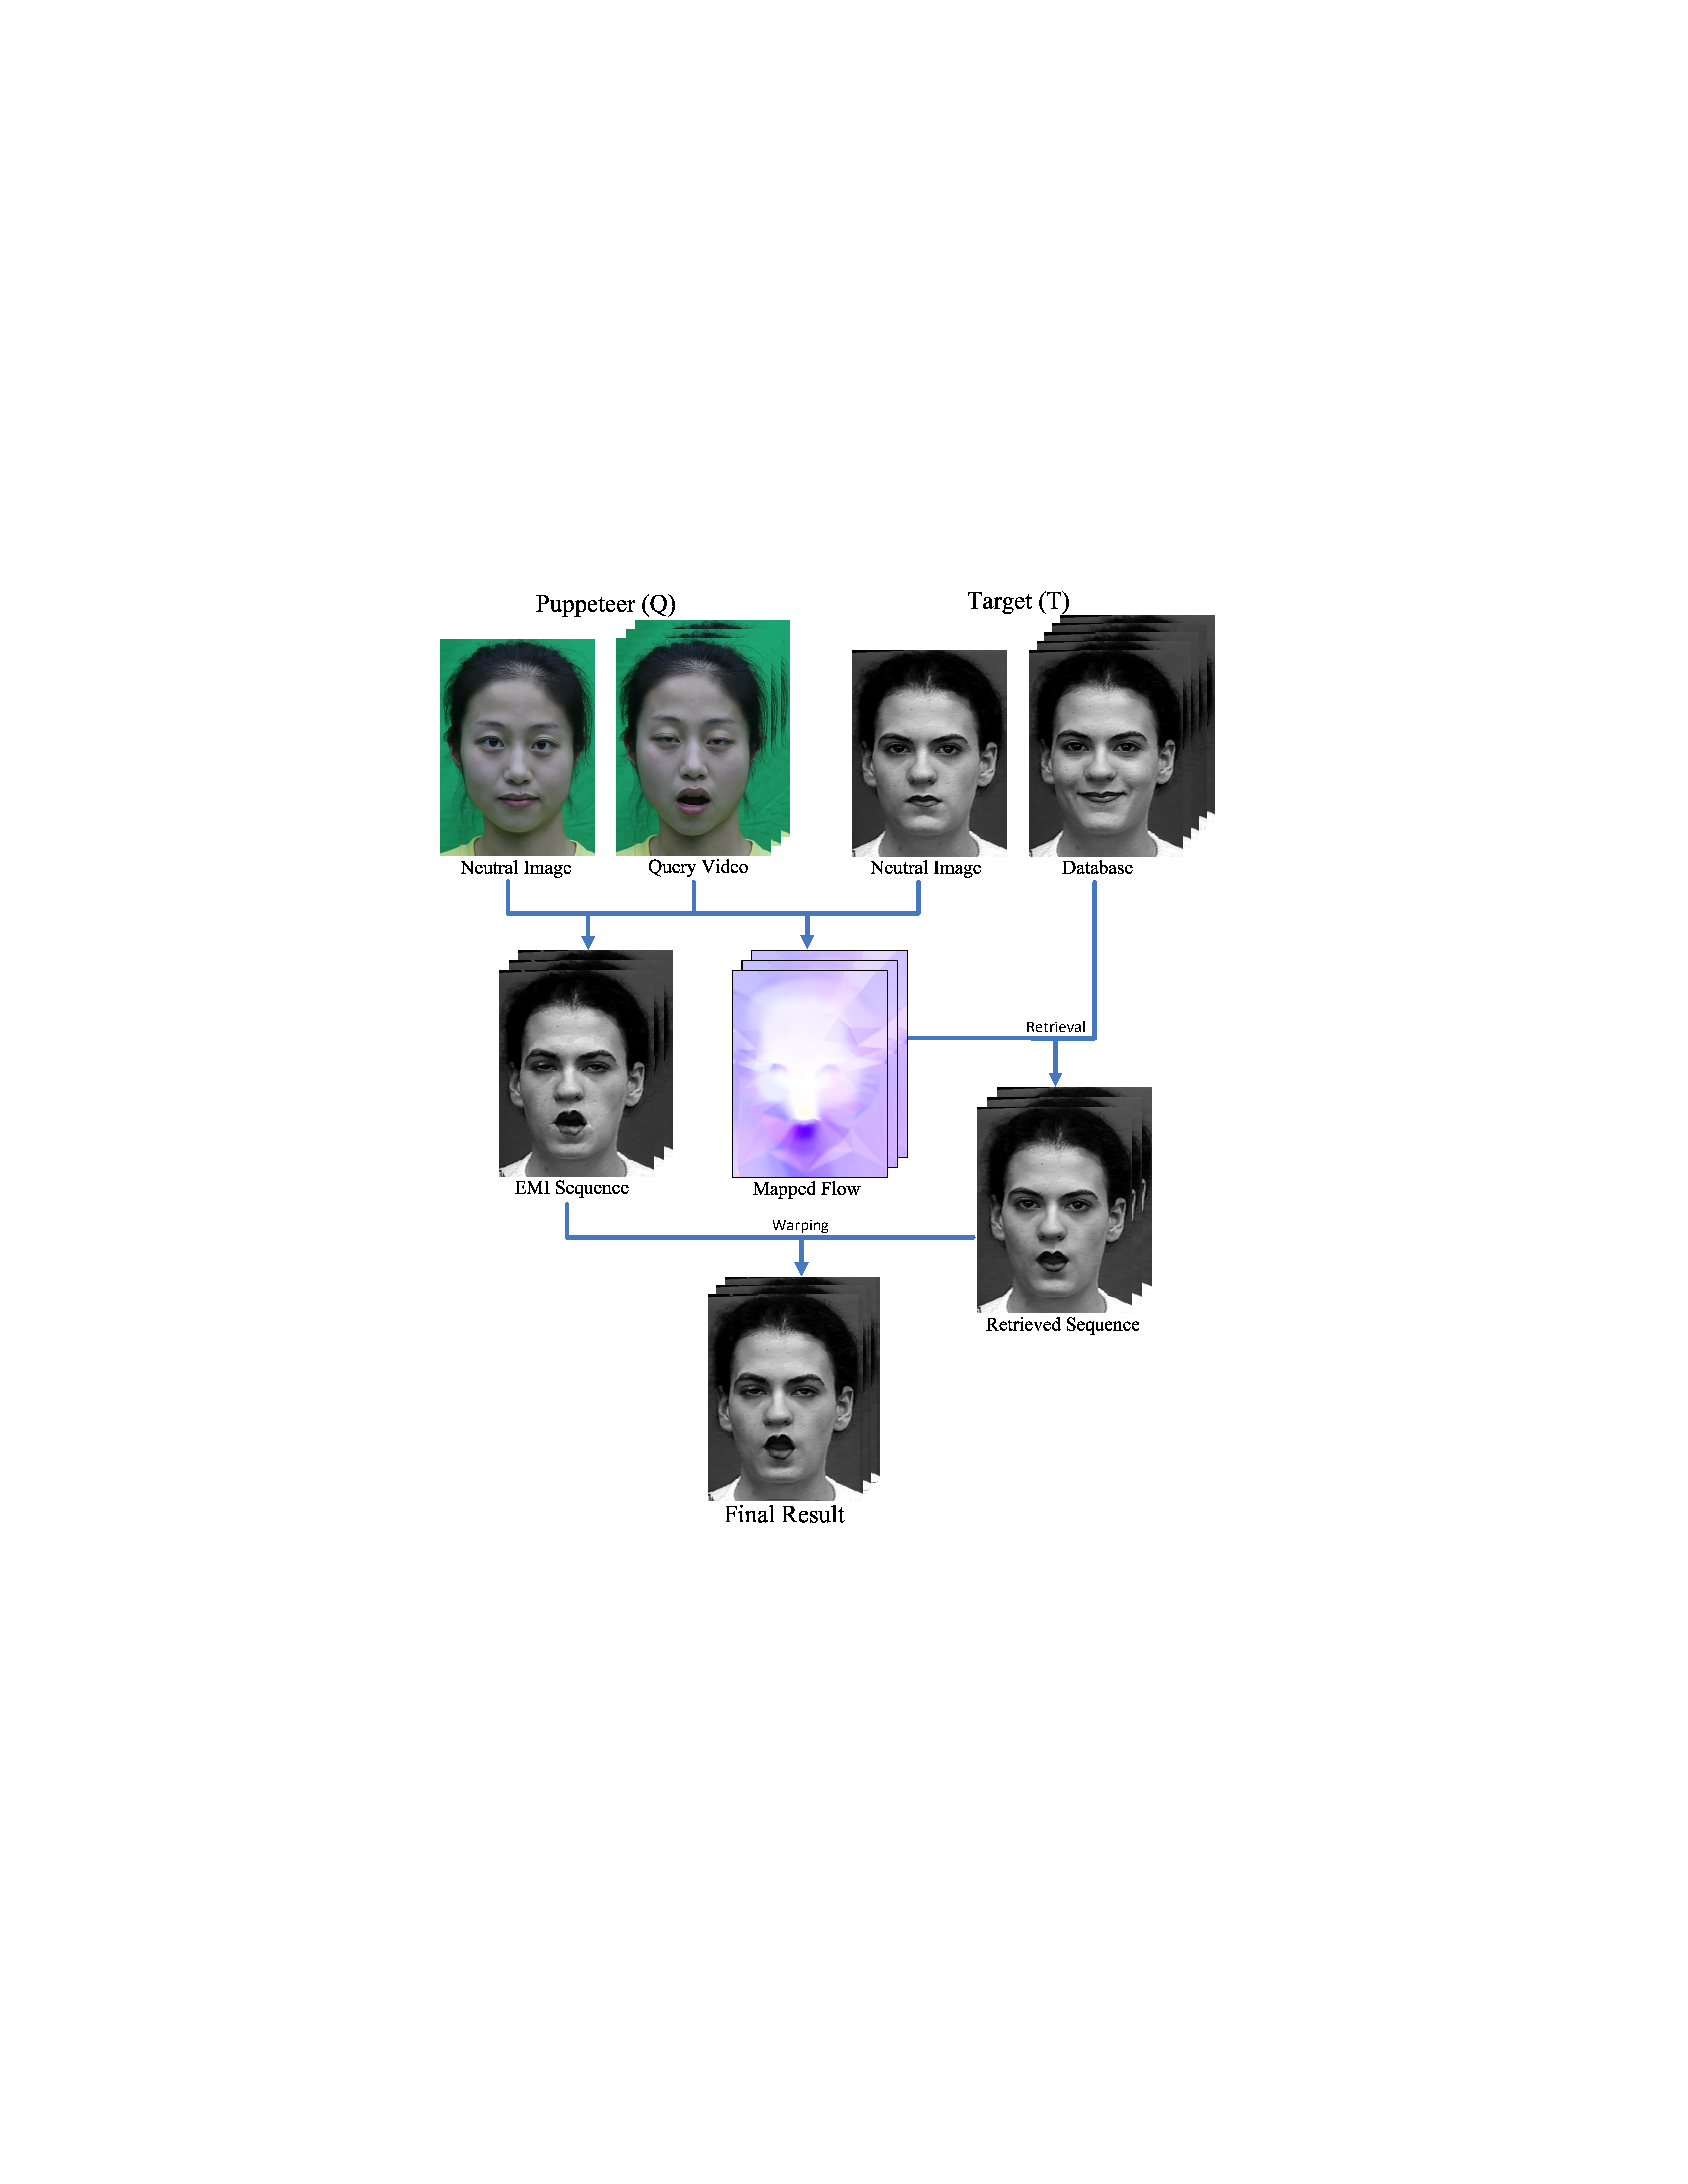
\includegraphics[width=0.95\textwidth]{data/img/overview.pdf}
    \caption{系统概览. 首先将每个查询帧和它的中性面部之间的光溜映射到目标人,用来从数据库中检索。同时,目标人的中性图像被扭曲以生成含有查询表情的EMI序列。最后,检索序列用EMI 精炼,来生成最终结果。}
    \label{fig:overview}
\end{figure}
图~\ref{fig:overview}展示了我们系统的概况。要为目标人生成逼真的表情,我们首先捕捉一段这个人展示基本表情的视频,比如生气、恐惧、惊奇、伤心、高兴、厌恶。有了另一个我们叫做人偶师(puppeteer)的人的面部表情,我们的方法尝试利用目标人的数据合成同样的表情。

具体而言,对于每个输入帧,我们使用第~\ref{sec:metric}章描述的基于光流相似度度量方法查询数据库获得$k$个与输入帧有最相近表情的目标人的视频帧。正如在第~\ref{sec:retrieval} 章描述的那样,我们把这个任务认为是和最短路问题一样找最优连续帧,而不是像Kemelmacher-Shlizerman等人~\cite{eccv10} 直接用最相似的帧生成一个匹配序列。获得的序列包含和人偶师相似且时间一致的表情。

然而,由于数据库大小有限,为每个输入帧找到一个完美的表情匹配几乎是不可能的,更何况,一些表情的人偶师具有独特的特点。为了考虑再输入和检索帧之间细微的表情差异,我们用一个表情映射技术来生成另一个候选面部,我们称之为EMI图像,如第~\ref{sec:emi}章描述那样。EMI图片通常有比检索帧有更精确的面部表情,但她的面部外观可能有重大瑕疵。在最后一步,我们把EMI图片和检索帧结合起来从而生成有精确表情和逼真外观的最终输出帧,如第~\ref{sec:emi}章所述。
\section{算法}
\subsection{表情相似度度量}\label{sec:metric}
给出人偶师的面部图片$Q_e$, 我们的系统试图从目标人的数据库中找到对应面部图片$T_e$,这幅图片有和$Q_e$最接近的面部表情. 为此我们需要能准确测量$Q_e$ 和 $T_e$之间表情差异的面部相似度度量, 同时忽视两幅图片的外表差异。

为了找到这样一个度量,我们的系统使用人偶师和目标人的中性面,分别记作$Q_n$ 和 $T_n$。当我们建立数据库的时候 $T_n$ 只需要标识一次,我们假设 $Q_n$ 在输入视频中由用户标记。为了说明人偶师的面部如何从 $Q_n$ 到 $Q_e$变化,我们能计算两幅图片中的光流场~\cite{celiu}记作 \mbox{\boldmath $F$}$_{Q_n \to Q_e}\in\mathbb{R}^{m \times 2}$, 这里$m$表示$Q_n$中的所有人脸像素。为了从光场中去除全局头部运动,我们用不随表情变化的鼻子区域来估计2D相似度变化,在计算表情差异前先把$Q_e$和$Q_n$对齐。我们也用脸的宽度归一化光流。类似的,$T_n$和$T_e$之间的光流场\mbox{\boldmath $F$}$_{T_n \to T_e}\in\mathbb{R}^{n \times 2}$, 其中$n \neq m$, 也可以计算。然而,由于身份/外观不同我们不能直接对比这两个光场。
\begin{figure}[htbp]
\centering
    \subcaptionbox{面部标记}{
    \label{fig:face_marker}
    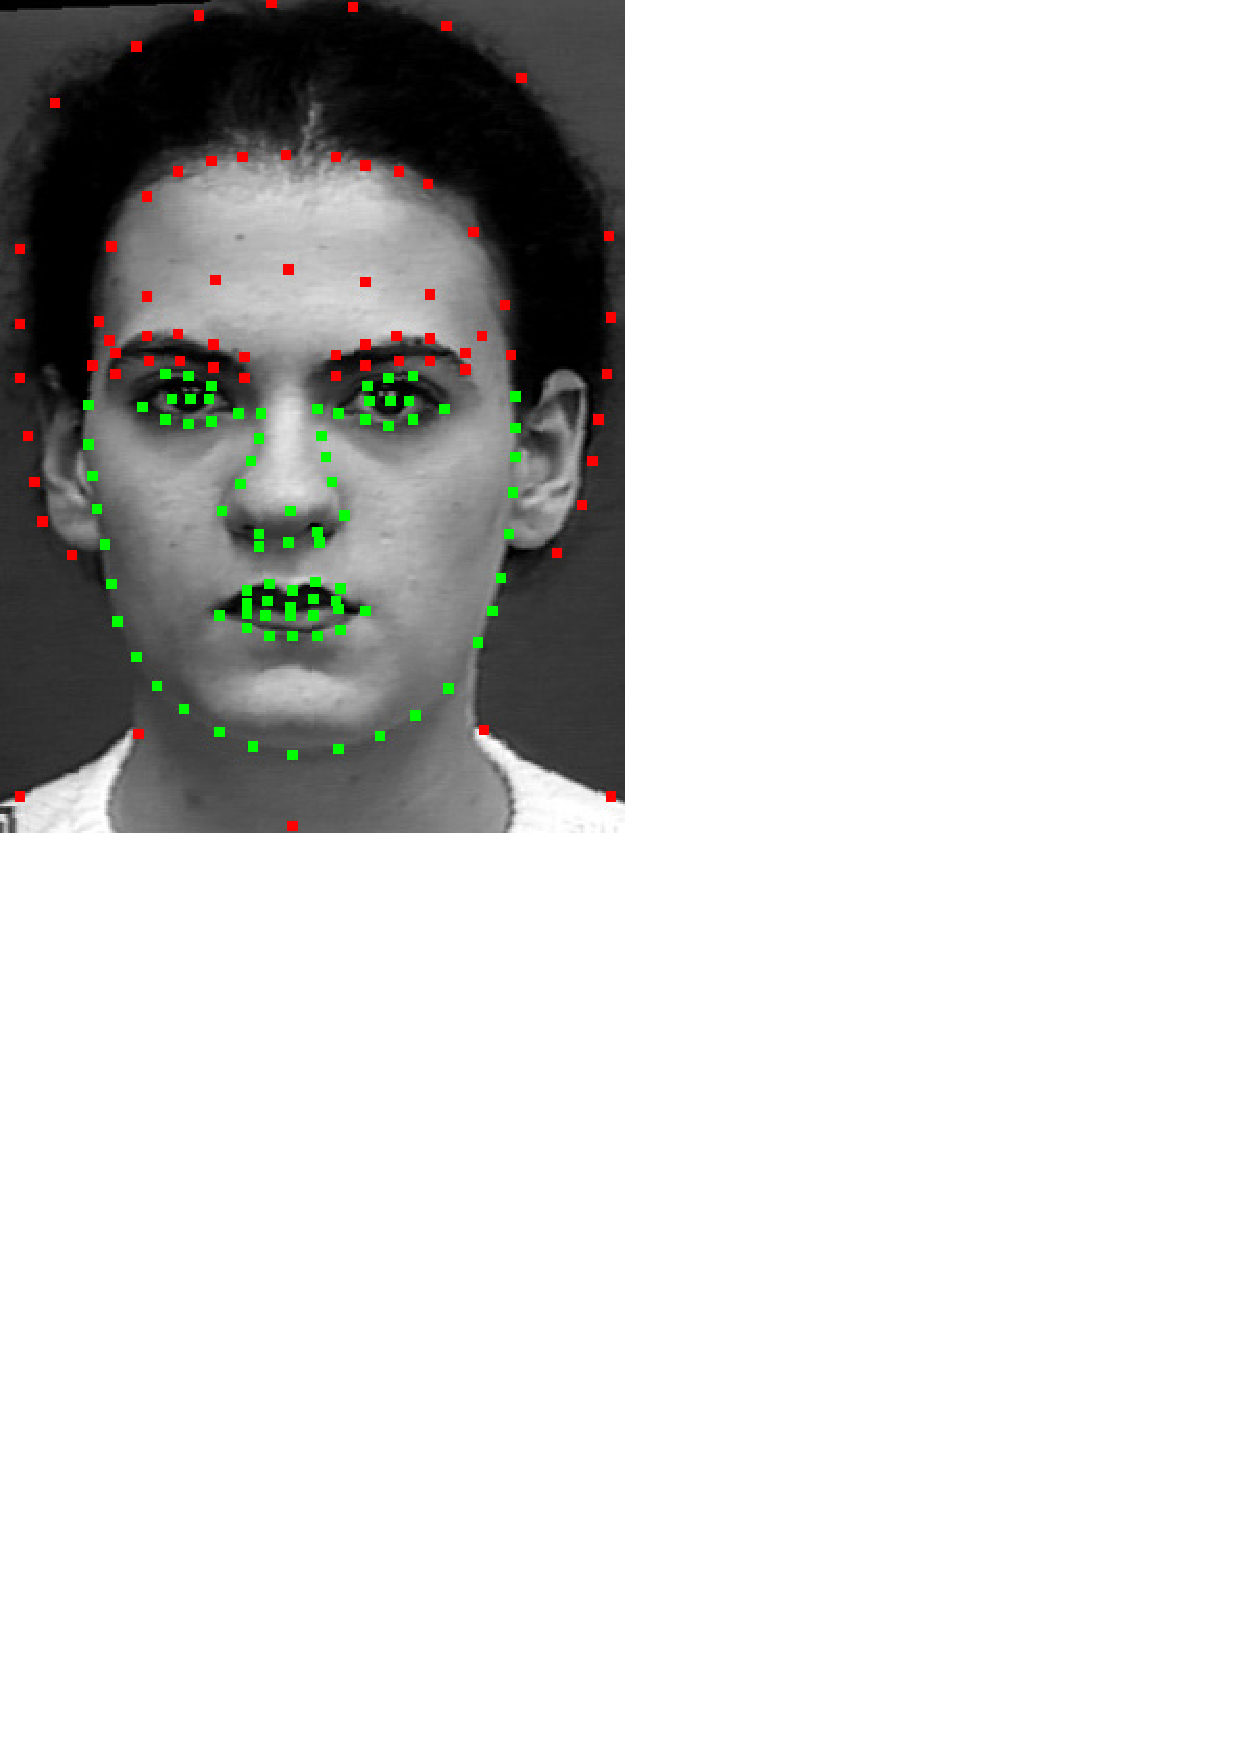
\includegraphics[width=0.20\textwidth]{data/img/facemarker.pdf}}
    \hspace{5mm}
    \subcaptionbox{局部区域}{
    \label{fig:face_region}
    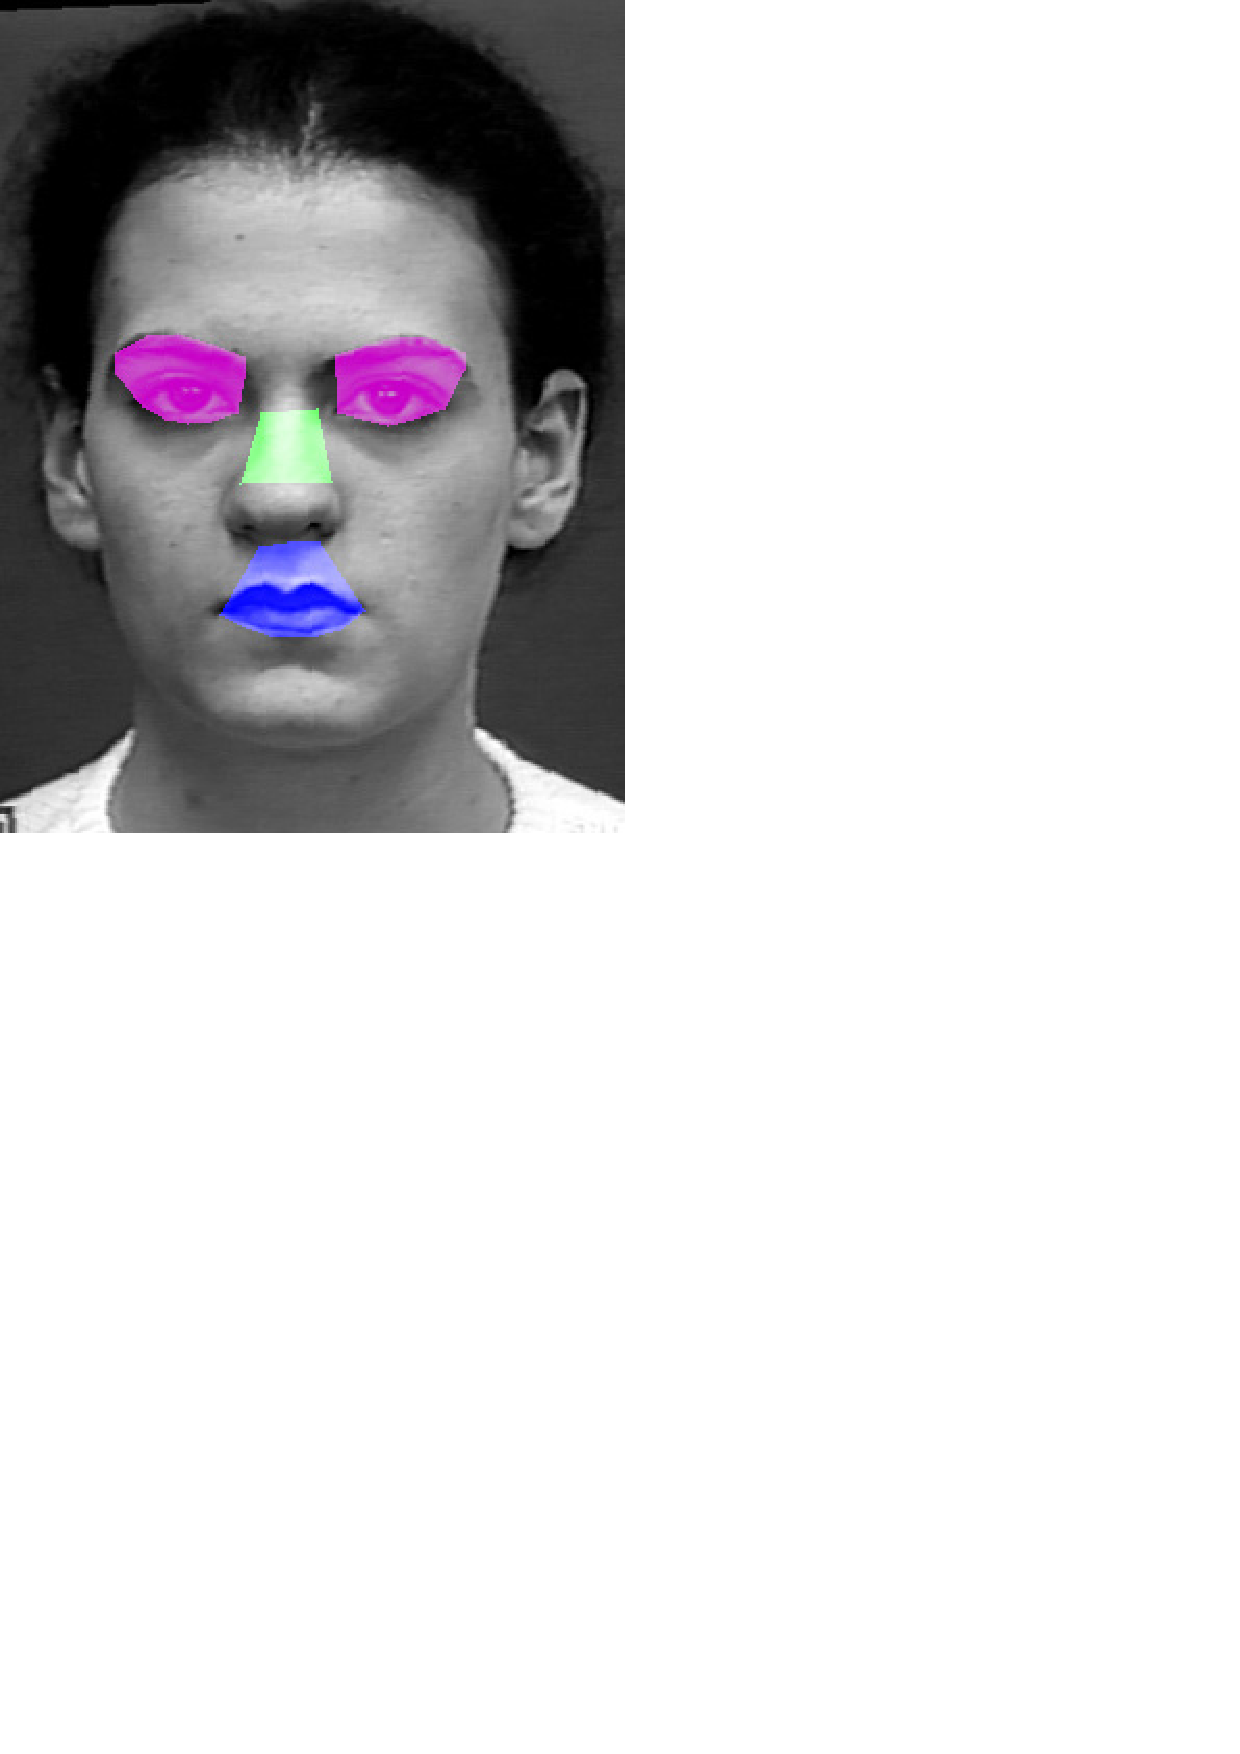
\includegraphics[width=0.20\textwidth]{data/img/faceregion.pdf}}
    \caption{中性脸初始化 (a) 绿色是ASM的标记,红色是手工标记
    (b) 眼睛、嘴巴、鼻子区域分别用品红、蓝色、绿色标记。}
    \label{fig:face}
\end{figure}
为了在两个光场之间建立精确的对应,我们首先使用Active Shape Model (ASM)~\cite{asm}只检测在中性面$Q_n$和$T_n$的面部标志物,该方法对于中性表情的正面人脸很有效。然而它无法覆盖我们算法在之后几步中需要的所有面部。因此我们在两个中性面上手工标注标志点,如图~\ref{fig:face_marker}所示。然后我们用Delauney三角网标出$Q_n$ 和 $T_n$ 中的脸部区域,这引出一个只能像素注册函数$g: Q_n \to T_n$。此外,由于两个身份之间的语义对应应该对不同的面部表情具有不变性,可以合理假设$g': Q_e \to T_e$两个表情图片的注册函数近似和$g: Q_n \to T_n$ 相同。有了注册函数,对于一个点$\vec{a}\in Q_n$转移到$\vec{a}' \in Q_e$,它在$T_n$对应的光流向量按如下计算:
\begin{equation}\label{eq:map2}
\Delta \vec{b}=g(\vec{a}')-g(\vec{a}),
\end{equation}
其中$\vec{b}=g(\vec{a})$是$T_n$上$\vec{a}$的对应点。

通过在$Q_n$上的所有面部像素应用这个映射,我们获取了一种映射好的光流场\mbox{\boldmath $F$}$'_{Q_n \to Q_e}$,可以通过与\mbox{\boldmath $F$}$'_{Q_n \to Q_e}$对比测量两个表情有多接近。以往工作指出~\cite{eccv10},表情差异的主要来源是眼睛和嘴巴区域,因此我们只用这些区域的像素来计算表情相似度(参见图~\ref{fig:face_region})。直接的方法是通过绝对的光流差计算$Q_e$ 和 $T_e$之间的表情差异:
\setlength\arraycolsep{1pt}
\begin{eqnarray}\label{eq:dist_mag}
d_e(Q_e, T_e)&=& \alpha_{e}\sum_{i\in\text{eye}}\left\|F'_{Q_n \to Q_e,i} -F_{T_n \to T_e,i}\right\| \nonumber\\
  &&+\alpha_{m}\sum_{i\in\text{mouth}}\left\|F'_{Q_n \to Q_e, i} -F_{T_n \to T_e, i}\right\|,
\end{eqnarray}

这里下标$i$表示光流矩阵\mbox{\boldmath $F$}中第$i$行。$\alpha_{\{e, m\}}$分别是眼睛和嘴巴区域的权重。
\begin{figure}[htbp]
\centering
    \subcaptionbox{}{
    \label{fig:metric_driven}
    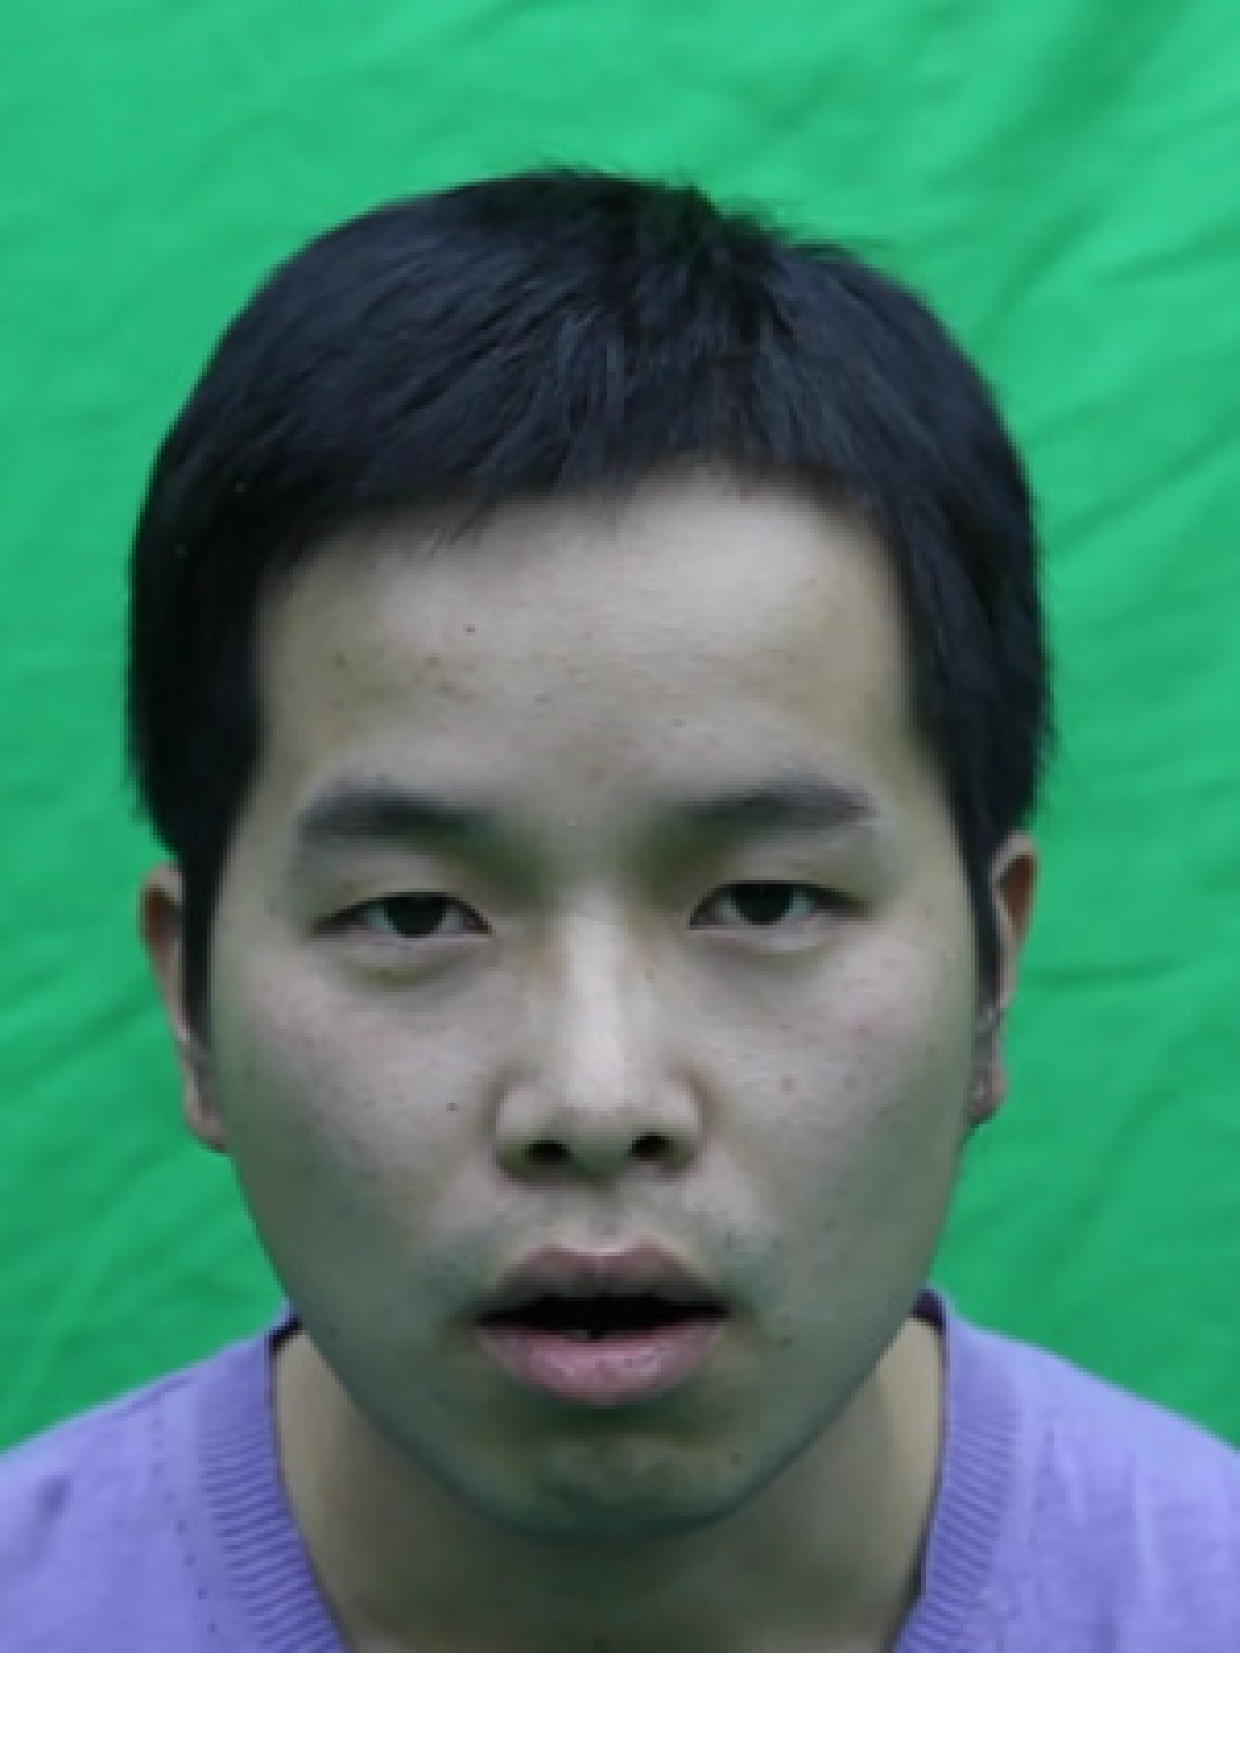
\includegraphics[width=0.2\textwidth]{data/img/metric_likai_0380_00103.pdf}}
    \subcaptionbox{}{
    \label{fig:metric_lbp}
    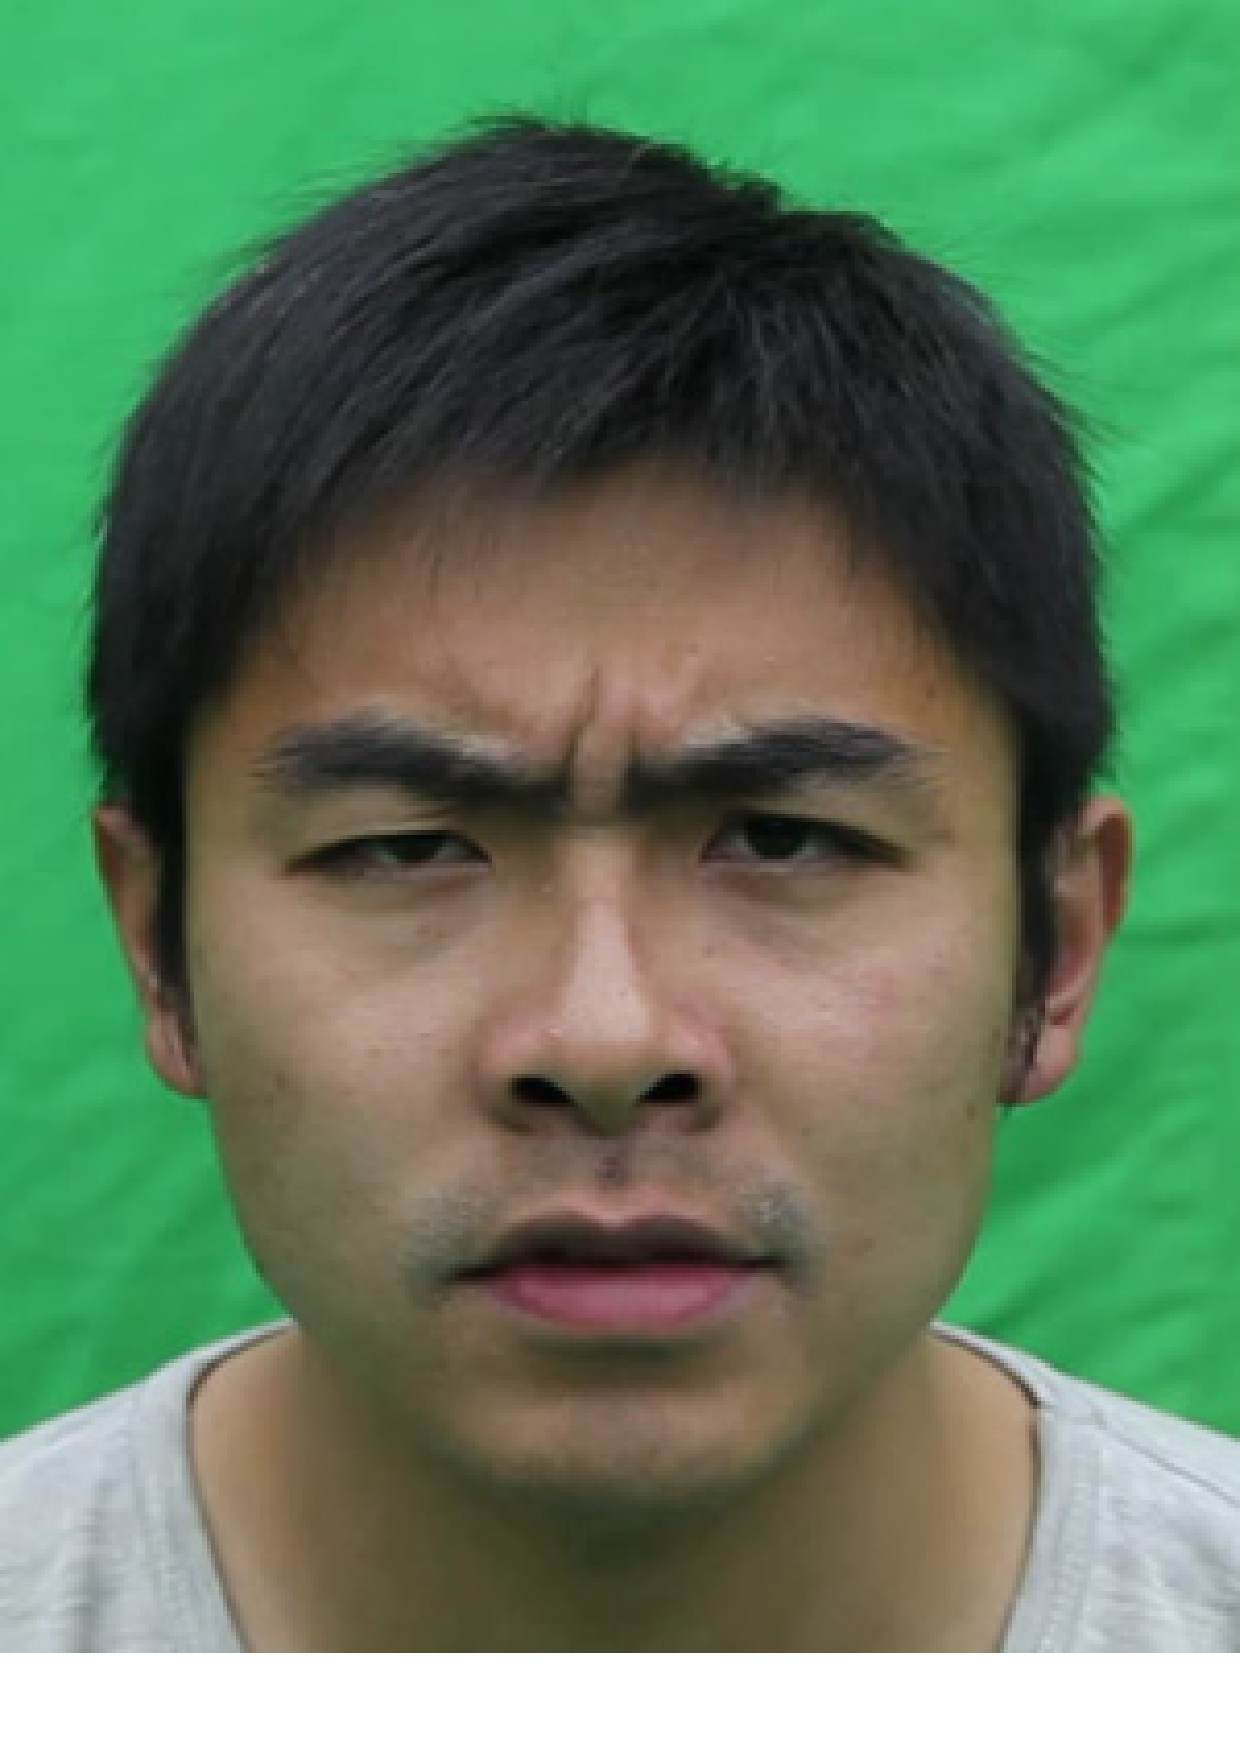
\includegraphics[width=0.2\textwidth]{data/img/metric_lbp_00102.pdf}}
    \subcaptionbox{}{
    \label{fig:metric_mag}
    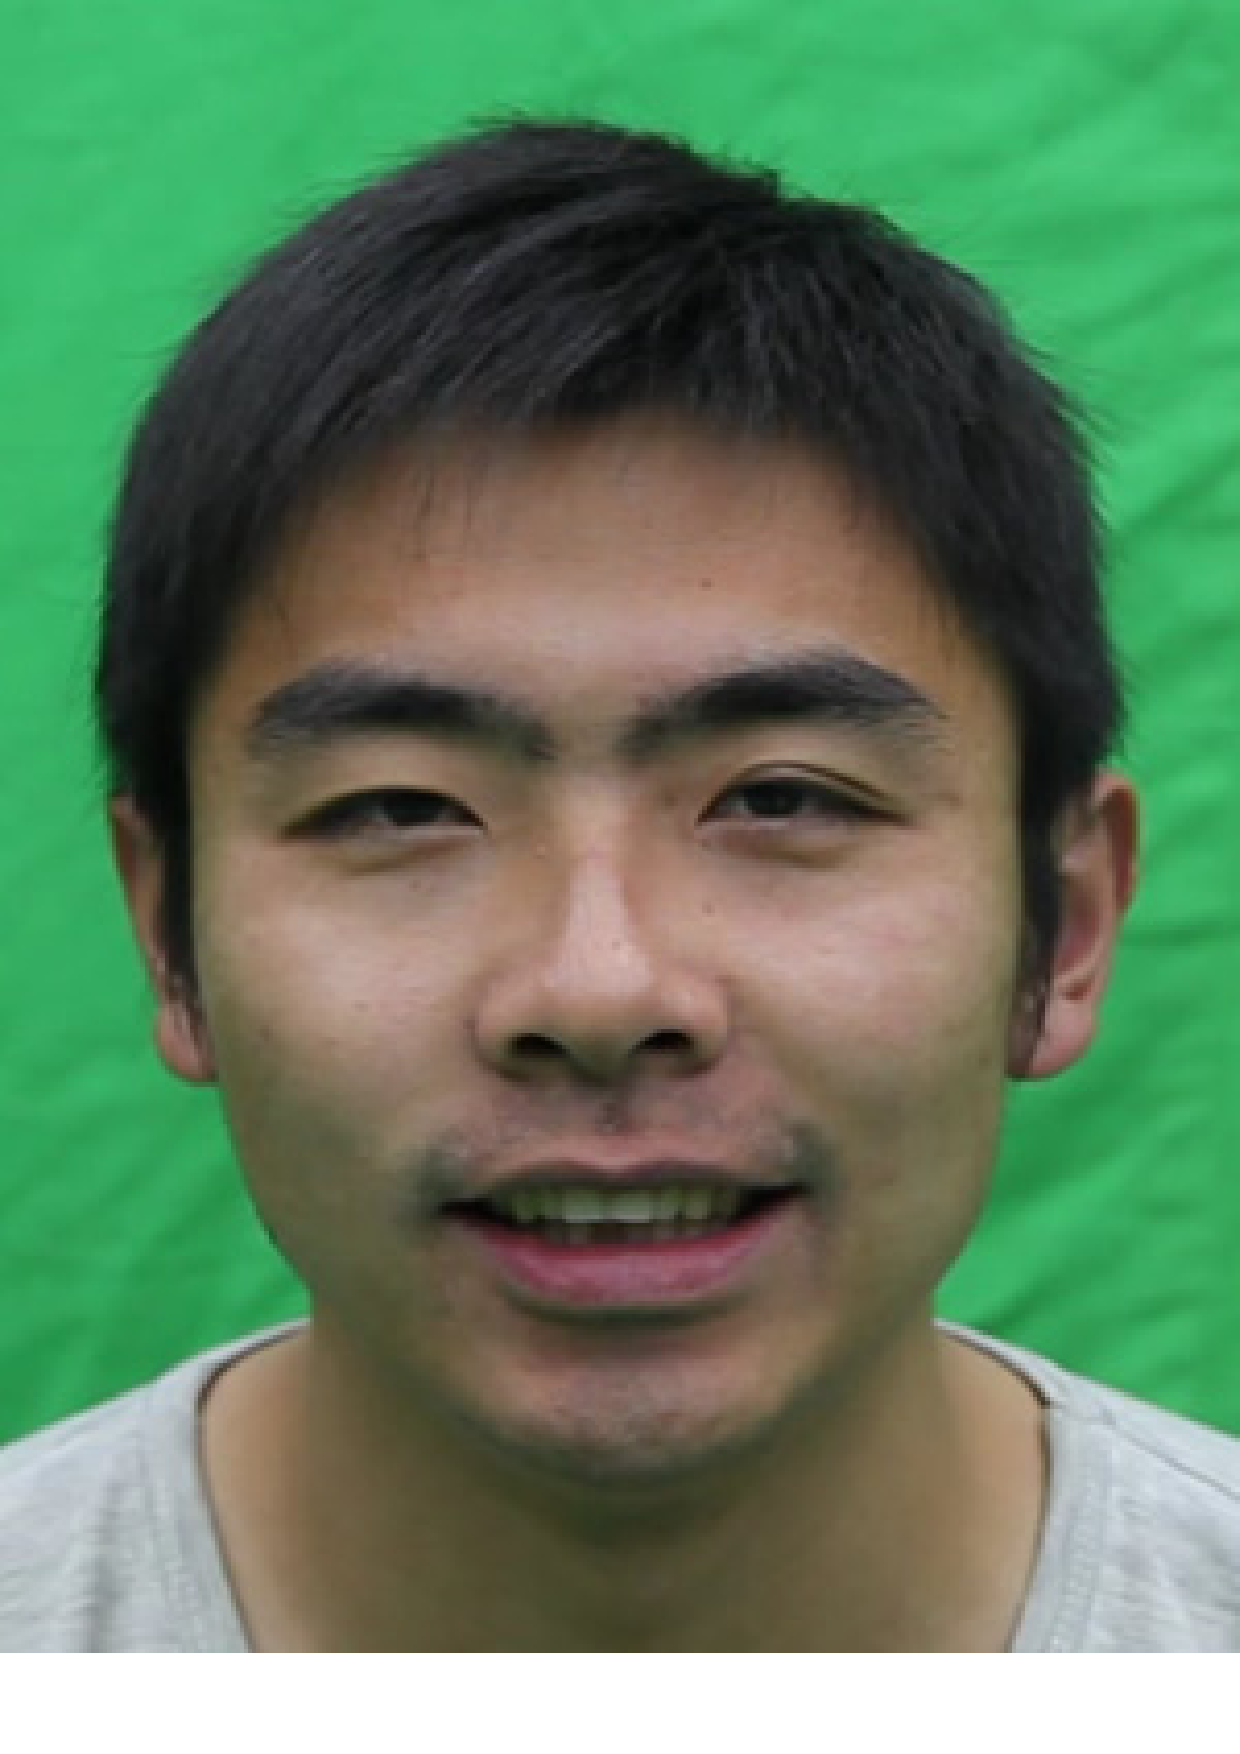
\includegraphics[width=0.2\textwidth]{data/img/metric_OFmag_00102.pdf}}
    \subcaptionbox{}{
    \label{fig:metric_magori}
    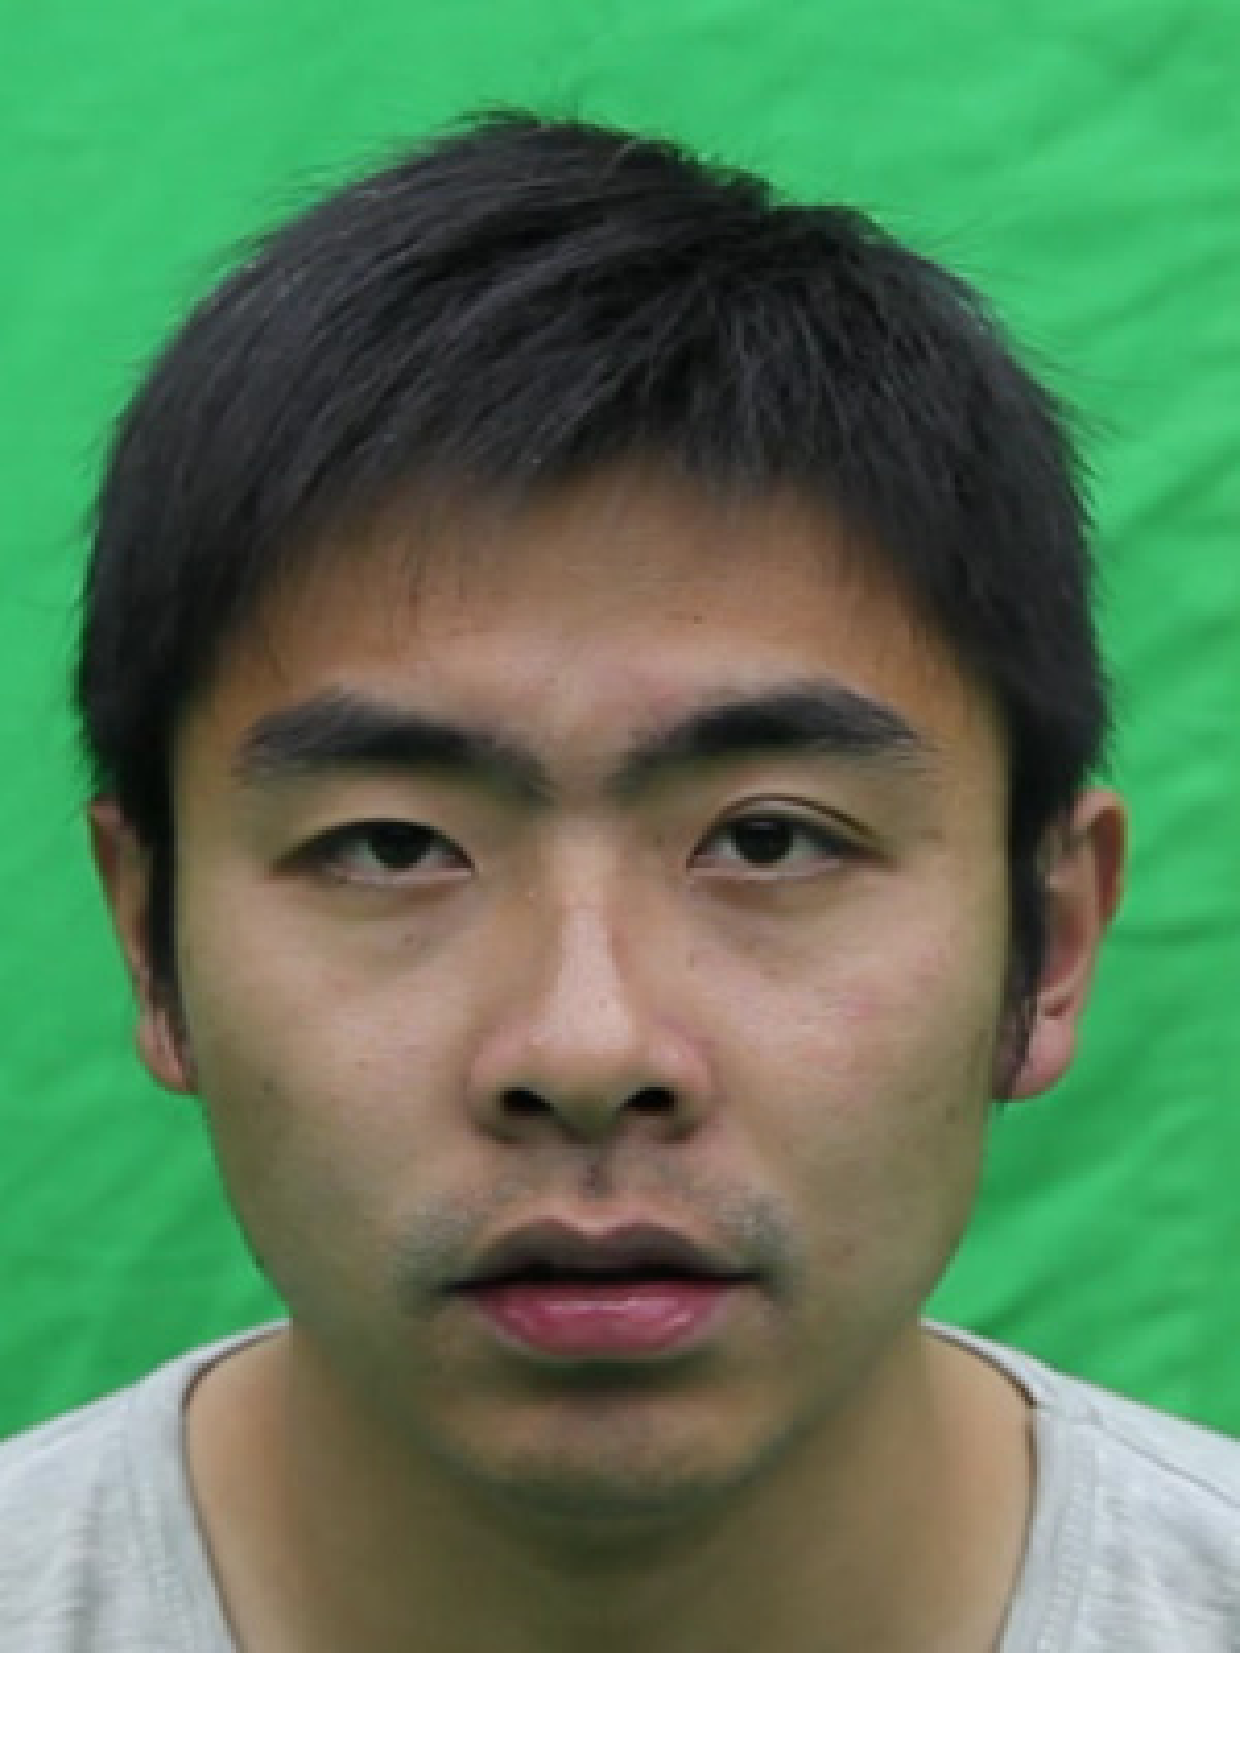
\includegraphics[width=0.2\textwidth]{data/img/metric_OFmagori_00102.pdf}}
    \caption{表情度量对比。 (a) 查询帧。 (b) 由LBP方法得到的最相似表情,它有一个不理想的皱眉。 (c) 由等式~\ref{eq:dist_mag}获得的最相似表情,有一个笑容而不是惊奇。 (d) 由等式~\ref{eq:dist_comb}获得的最相似表情,和查询帧匹配很好}
    \label{fig:metric}
\end{figure}

等式~\ref{eq:dist_mag}中的距离度量在我们大多数实验中都很成功,但我们发现会偶尔产生如图~\ref{fig:metric}所示的错误。这是因为在等式~\ref{eq:dist_mag}中,我们仅考虑了\mbox{\boldmath $F$}$'_{Q_n \to Q_e}-$\mbox{\boldmath $F$}$_{T_n \to T_e}$的光流差异的大小。但光流的方向通常包含更多有关表情的重要信息。比如笑脸通常与嘴角的上翘相关,而哭脸和嘴角下弯相关。这表明在$Q_e$中的表情与$T_e$中的很不一样,如果\mbox{\boldmath $F$}$'_{Q_n \to Q_e}$到\mbox{\boldmath $F$}$_{T_n \to T_e}$的差异方向很不一样,即便差异大小很小。有了这个发现,我们重新设计表情距离度量如下:
\setlength\arraycolsep{1pt}
\begin{eqnarray}
d_b(\vec{u},\vec{v})&=&\beta_m|\vec{u}-\vec{v}|+\beta_o(-\vec{u}\cdot\vec{v}+|\vec{u}||\vec{v}|), \label{eq:d0}\\
d_e(Q_e, T_e)&=&\alpha_{e}\sum_{i\in\text{eye}}d_b(F'_{Q_n \to Q_e,i}, F_{T_n \to T_e,i})\nonumber\\
           &&+\alpha_{m}\sum_{i\in\text{mouth}}d_b(F'_{Q_n \to Q_e, i}, F_{T_n \to T_e, i}),\label{eq:dist_comb}
\end{eqnarray}

这里$\beta_{\{m, o\}}\in[0,1]$分别是大小和方向的权重,且$\beta_m+\beta_o=1$。 当$\beta_o$ 等于零,等式~\ref{eq:dist_comb}简化为等式~\ref{eq:dist_mag}。在等式~\ref{eq:d0} 中的偏移量$|\vec{u}||\vec{v}|$确保方向项非负。注意此距离度量不保证对称性和三角不等式。为使之更有数学味,可以计算反向距离$d_e(T_e,Q_e)$,用二者平均值作为最终距离度量。但实际上我们发现这并无必要,因为$d_e(Q_e, T_e)$已很好描述不同身份两张图片的表情差异,对我们的应用而言已足够。
\subsection{基于检索的视频合成}\label{sec:retrieval}
使用如上定义的相似性度量,一个视频合成的简单方法是为每个输入帧,找到其在数据库中的最近邻表清,并叠在一起,以形成最终的输出视频。然而,我们发现这种方法并不很好,在最终视频中面部表情的时间相干性没有得到很好的保持,并且最终的视频经常出现抖动。补充材料包含了说明此问题的视频。我们的系统采用了一些额外的技术来解决的时间一致性问题,我们将在本小节详细介绍。
\subsubsection{结合表情速度}
首先,在公式~\ref{eq:dist_comb}中定义的距离度量只考虑了两个面部的表情相似度。然而在视频中,我们需要关心在每一帧表情变化的速度。最相似的帧应该是表情及其变化速度都与查询帧相符的。为了保证表情速度,我们在视频序列中简单地计算另一个在当前帧和下一帧之间的光流。记$Q_e^{(q)}$为第 $q$个查询帧,表情速度计算如下:
\begin{equation}\label{eq:dF_Q}
\text{d} \mbox{\boldmath $F$}_{Q_e^{(q)}} = \mbox{\boldmath $F$}_{Q_e^{(q)}\to Q_e^{(q+1)}}.
\end{equation}

类似的,对于在数据库中的帧$T_e^{(t)}$,我们计算表情速度为d\mbox{\boldmath $F$}$_{T_e^{(t)}}$。同样,由于$Q_e^{(q)}$ 和 $T_e^{(t)}$身份和表情差异,直接计算d\mbox{\boldmath $F$}$_{Q_e^{(q)}}$ 和 d\mbox{\boldmath $F$}$_{T_e^{(t)}}$ 距离并不好。需要扭曲表情速度光流场来去除身份差异,如我们在
第~\ref{sec:metric}章所做。我们还需要扭曲两者的速度光流场来把他们映射到中性表情,以去除他们的表情差异。

具体说,对于数据库帧,我们把\mbox{\boldmath $F$}$_{T_n\to T_e^{(t)}}$的反向光流用于 d\mbox{\boldmath $F$}$_{T_e^{(t)}}$,导出与中性表情$T_n$相符的扭曲的表情速度流d\mbox{\boldmath $F$}$'_{T_e^{(t)}}$。对于查询帧$Q_e^{(q)}$,我们把公式~\ref{eq:dist_comb} 计算的反向光流\mbox{\boldmath $F$}$'_{Q_n\to Q_e^{(q)}}$用于d\mbox{\boldmath $F$}$_{Q_e^{(q)}}$,导出与中性表情$T_n$相符的扭曲的表情速度流d\mbox{\boldmath $F$}$'_{Q_e^{(q)}}$。最后,$Q_e^{(q)}$ 和 $T_e^{(t)}$的表情速度差异计算如下:
\begin{eqnarray}\label{eq:dist_deri}
d_v(Q_e^{(q)}, T_e^{(t)})&=& \alpha_{e}\sum_{i\in\text{eye}}d_b(\text{d}F'_{Q_e^{(q)}, i}, \text{d}F'_{T_e^{(t)}, i})\nonumber\\
           &&+\alpha_{m}\sum_{i\in\text{mouth}}d_b(\text{d}F'_{Q_e^{(q)}, i}, \text{d}F'_{T_e^{(t)}, i}),
\end{eqnarray}

此处函数$d_b(\cdot,\cdot)$在公式~\ref{eq:d0}中定义。结合公式~\ref{eq:dist_comb}和公式\ref{eq:dist_deri},最终的视频表情距离度量定义如下:
\begin{equation}\label{eq:dist_all}
\mathcal{D}(Q_e^{(q)}, T_e^{(t)})=\gamma_e d_e(Q_e^{(q)}, T_e^{(t)})+ \gamma_v d_v(Q_e^{(q)}, T_e^{(t)}),
\end{equation}

这里$\gamma_{\{e,v\}}\in[0,1]$分别是表情距离和表情速度距离的权重,满足$\gamma_e+\gamma_v=1$。

图~\ref{fig:velocity}的例子表明,当表情很微妙,在度量中结合表情速度能帮助系统更好的捕捉表情变化。
\begin{figure}[htbp]
\centering
    \subcaptionbox{}{
    \label{fig:velocity_driven}
    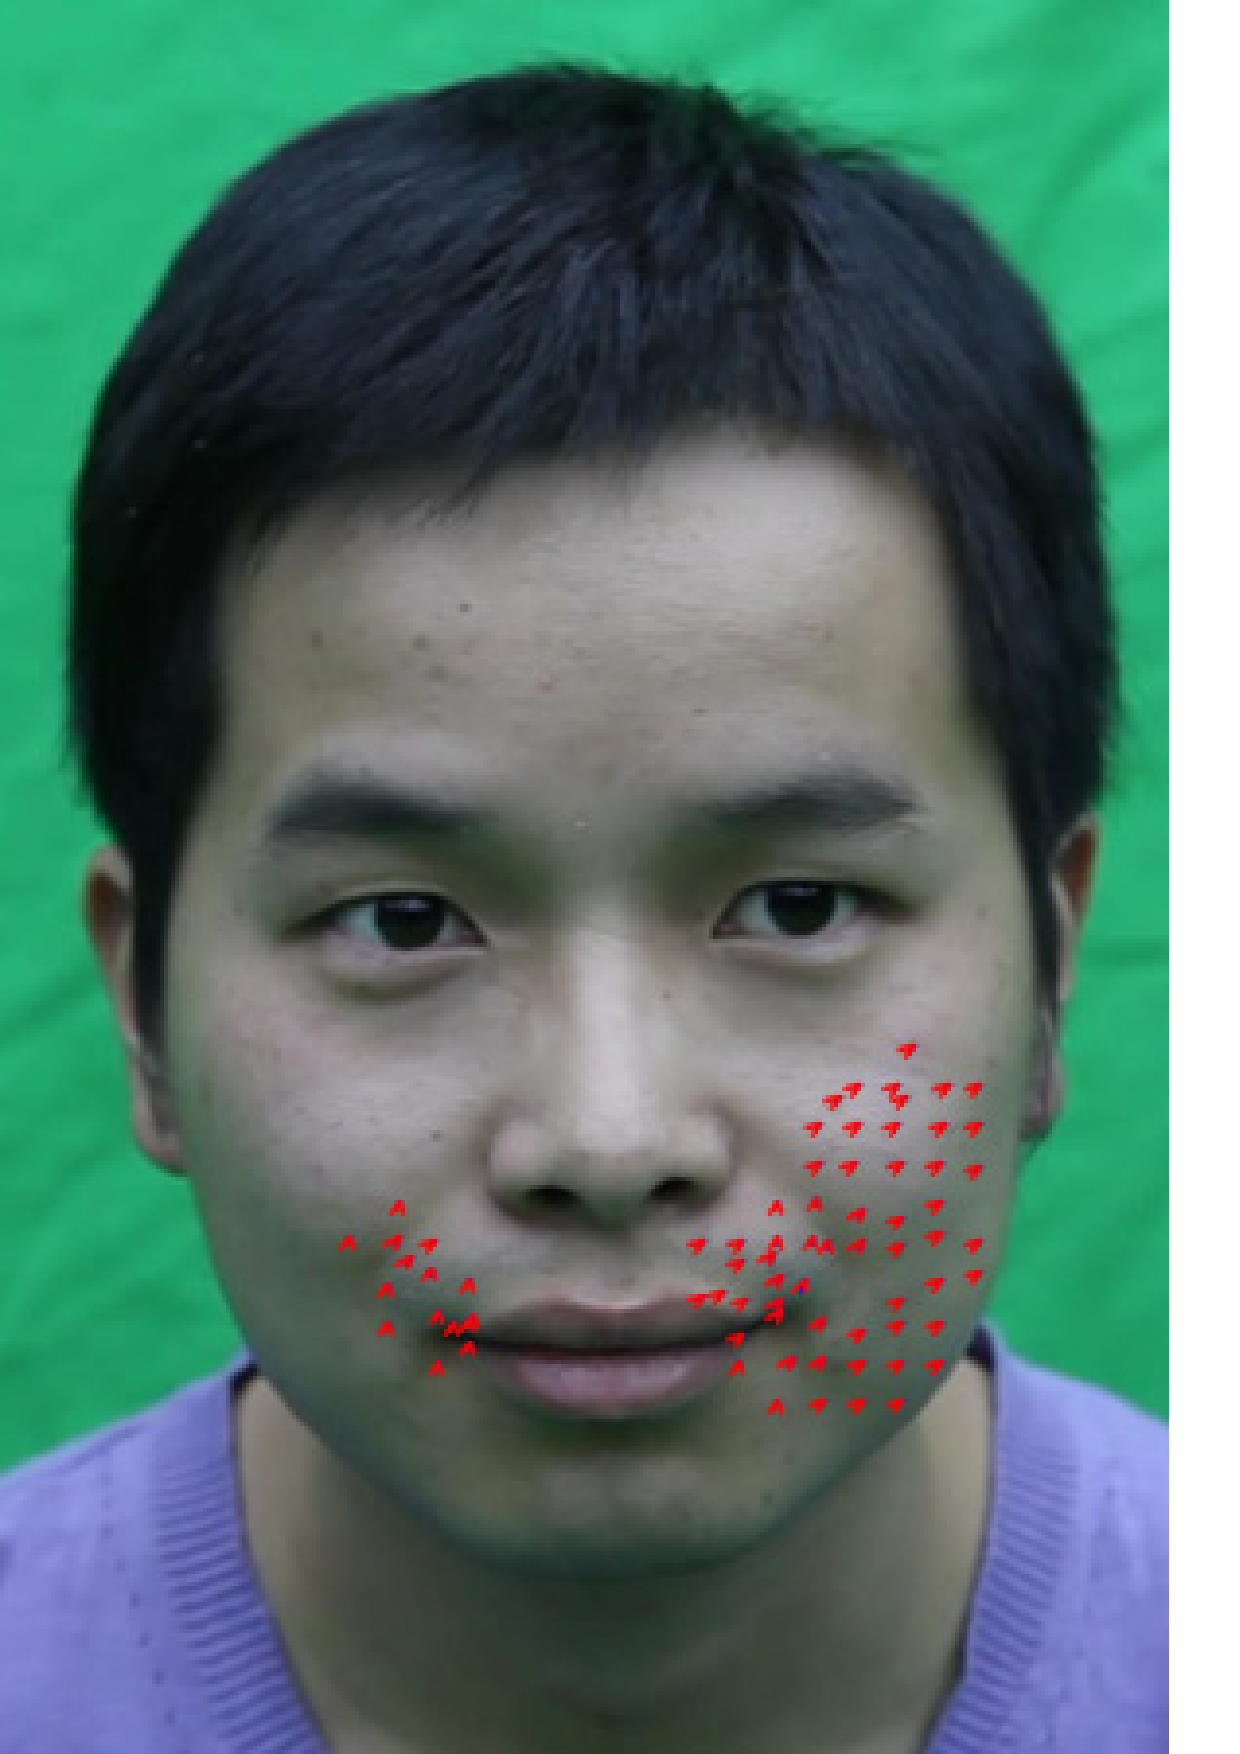
\includegraphics[width=0.205\textwidth]{data/img/velocity_likai_0380_00199_flow.pdf}}
    \subcaptionbox{}{
    \label{fig:velocity_next}
    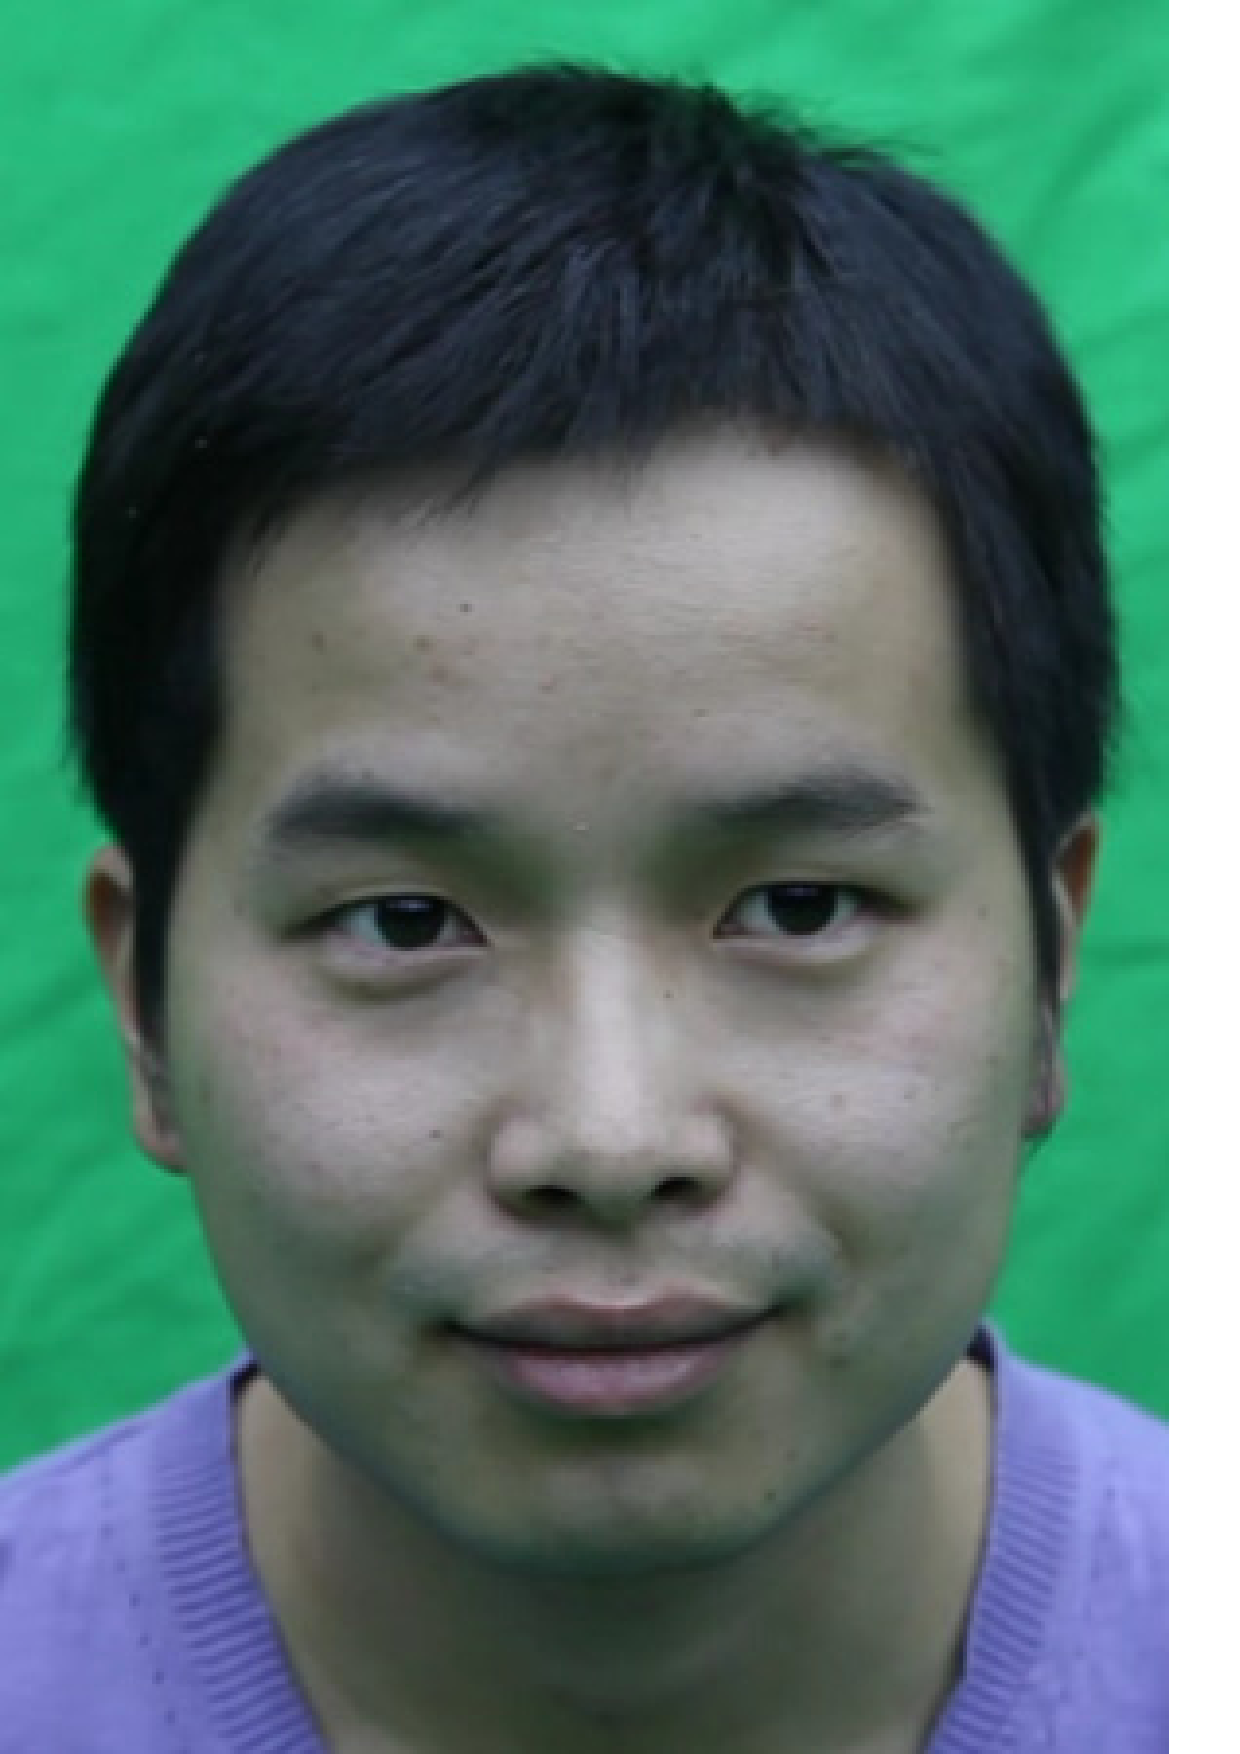
\includegraphics[width=0.205\textwidth]{data/img/velocity_likai_0380_00200.pdf}}
    \subcaptionbox{}{
    \label{fig:velocity_without}
    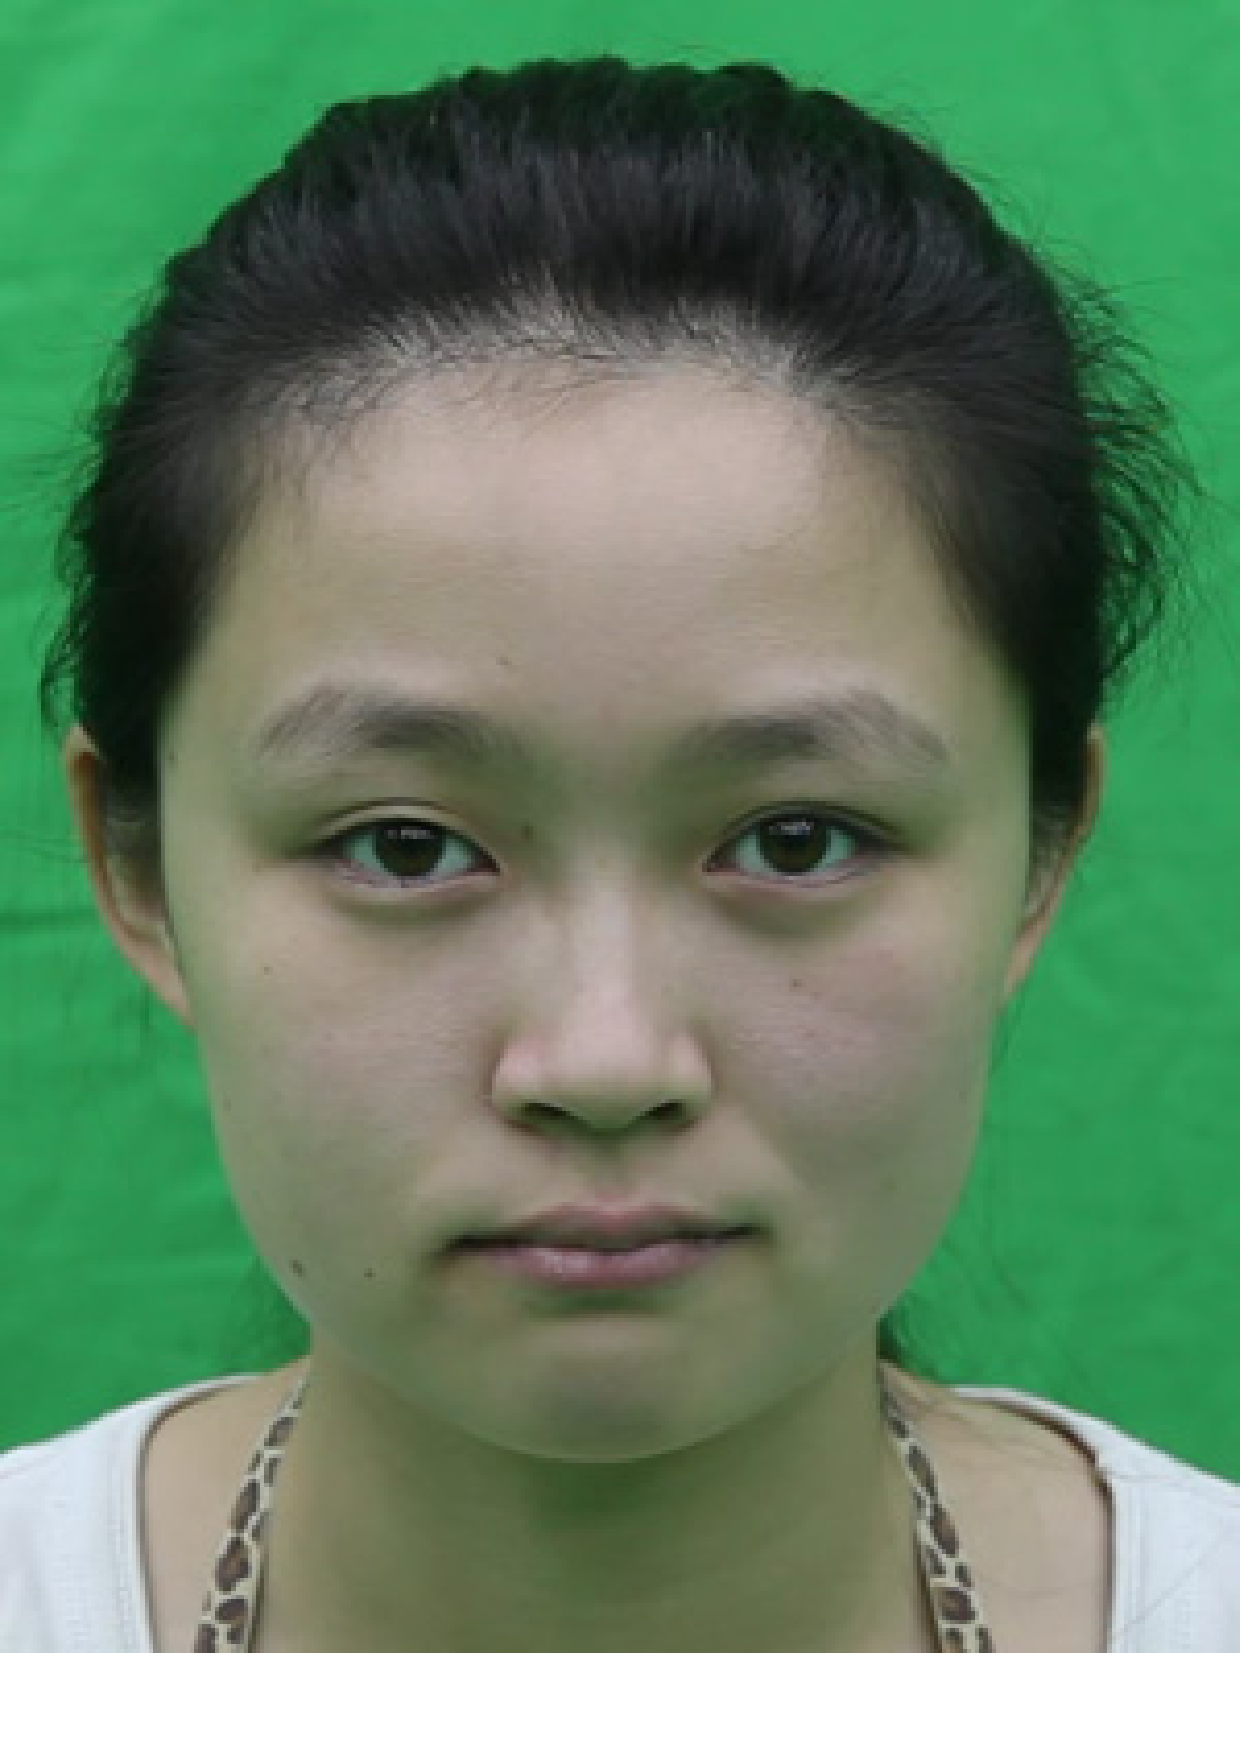
\includegraphics[width=0.23\textwidth]{data/img/velocity_without_00198.pdf}}
    \subcaptionbox{}{
    \label{fig:velocity_with}
    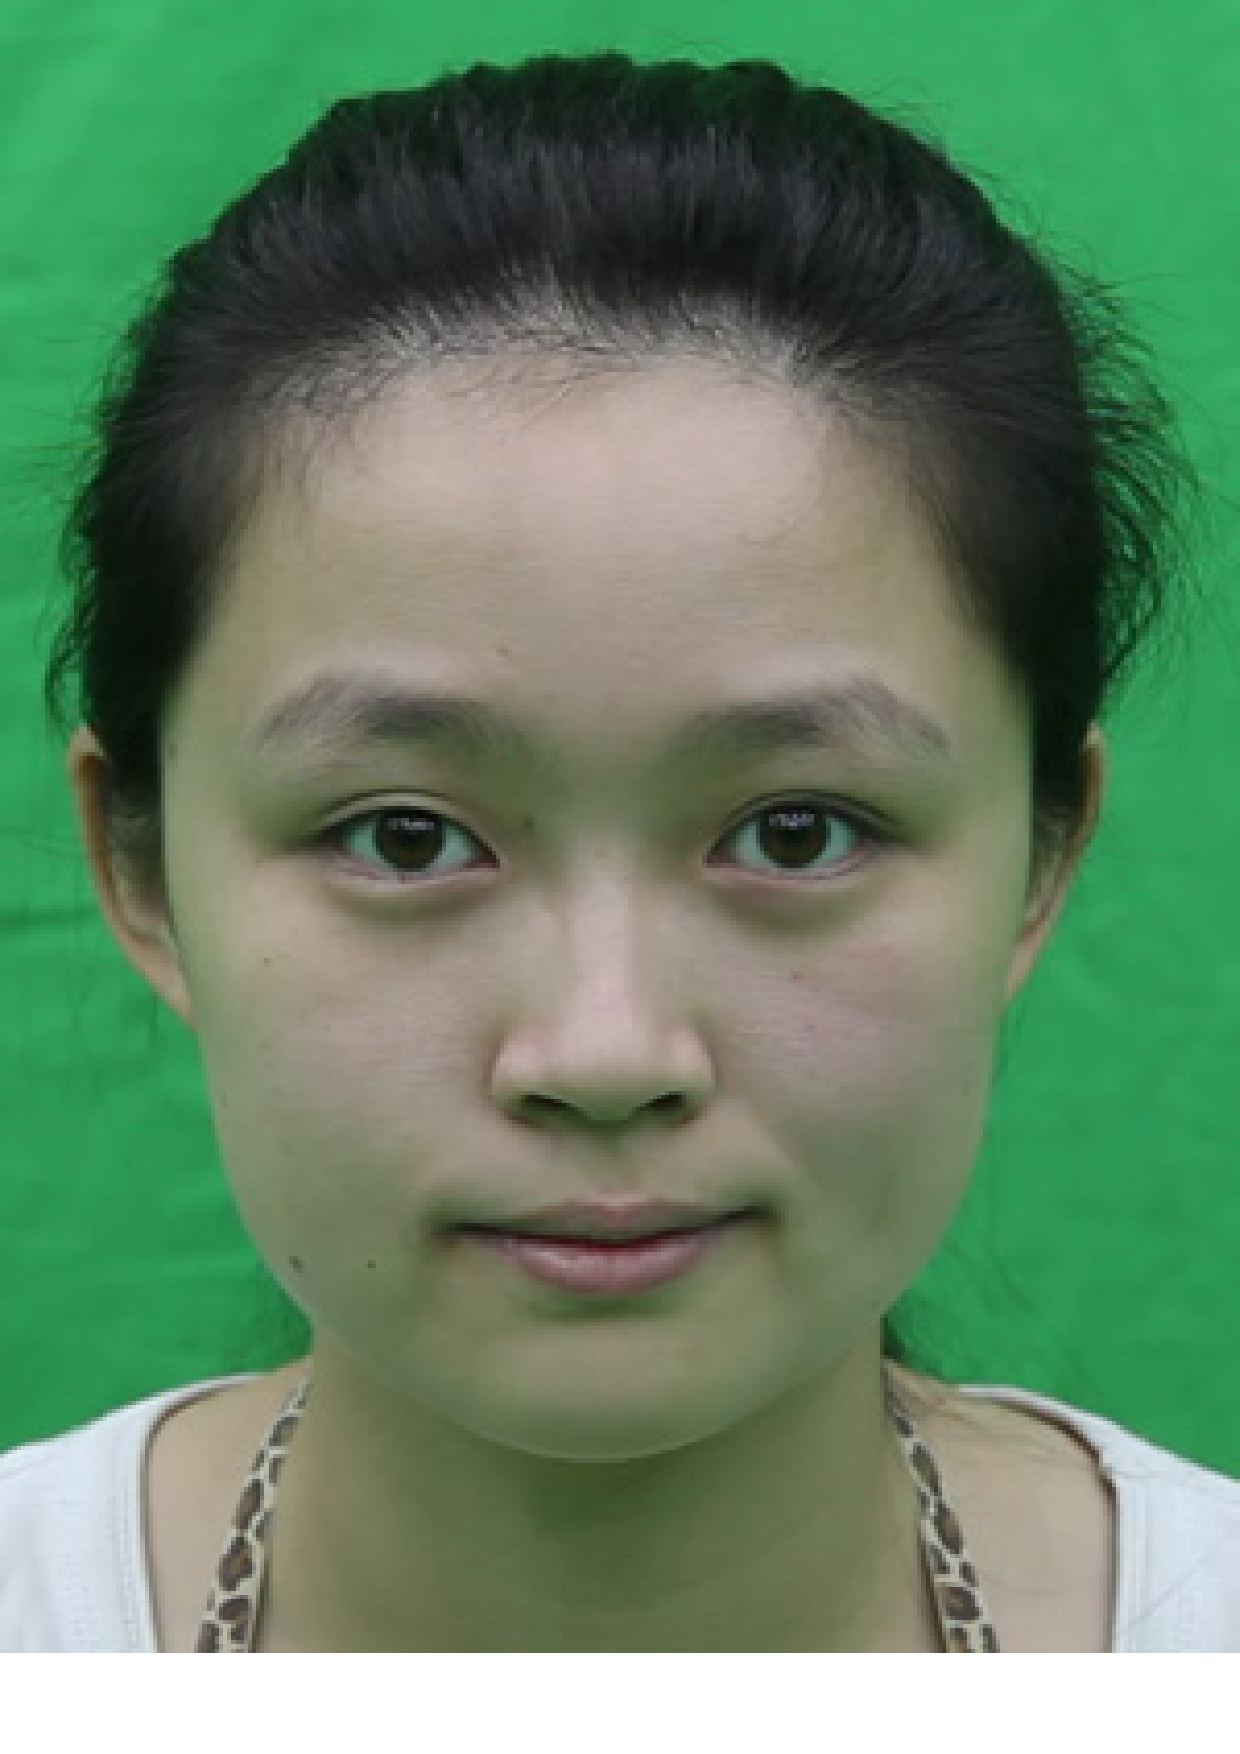
\includegraphics[width=0.23\textwidth]{data/img/velocity_with_00198.pdf}}
    \caption{使用表情速度的重要性阐述。(a) 红色表示带表情速度的当前查询帧。(b) 微笑的下一查询帧。(c) 由公式~\ref{eq:dist_comb}选择的最相似帧,有细淡淡的忧伤。(d)由公式~\ref{eq:dist_all}选择的最相似帧,有正确的微笑。}
    \label{fig:velocity}
\end{figure}

\subsubsection{基于优化的检索}
改进的表情相似度度量不能独立完整地解决时间一致性的问题。因此我们的系统使用就与优化的检索方法进一步提升合成序列的时间一致性。

对于每个查询帧,我们首先使用公式~\ref{eq:dist_all}定义的完整的距离度量从数据库不是抽取一个,而是$k$近邻,我们称之为候选帧。在每帧的时间戳放置一列$k$个候选帧,我们建立如图~\ref{fig:dijkstra}所示的有向无环图。有向边只连接邻近候选帧。记$V_i^{(q)}$ 为时刻$q$ 的第$i$候选帧。我们定义有向弧$r=(V_i^{(q)}, V_j^{(q+1)})$的长度为:
\begin{eqnarray}\label{eq:length}
\mathcal{L}(r)&=&\mathcal{D}(V_i^{(q)},Q_e^{(q)})+
        \mathcal{D}(V_j^{(q+1)},Q_e^{(q+1)})\nonumber\\
        &&+\lambda \exp ( - {{(\mathcal{T}(V_j^{(q + 1)} ) - \mathcal{T}(V_i^{(q)} ) - \mu )^2 }}/{{\sigma ^2 }}),
\end{eqnarray}

这里$\mathcal{T}(\cdot)$是输入帧的时间戳。通过最小化相邻帧的时间差,公式~\ref{eq:length} 的最后一项鼓励数据库中的连续帧选为匹配帧,以保证时间一致性。时间尺度变量$\mu$ 用于补偿查询和数据库序列之间的运动速度差。当查询帧和数据库序列运动速度大致相同,$\mu$设为1,当查询帧运动速度比数据库序列快则设为一个大数,否则相反。$\sigma$是带宽,$\lambda$是时间项的权重。

在公式~\ref{eq:length}中的时间项是L2范数,允许晓得时间变化,但对大的变化有严惩。由于小的变化被允许,它也允许某些时间尺度的变化。这在我们的查询序列1中被证明,如图~\ref{fig:result12}所示,它包含缓慢嘴巴张开的表情和快速撅嘴的表情。我们的系统对这二者都处理很好。此外,$\mu$也能在视频的不同时间根据查询运动的速度自动调整。

\begin{figure}[htbp]
\centering
    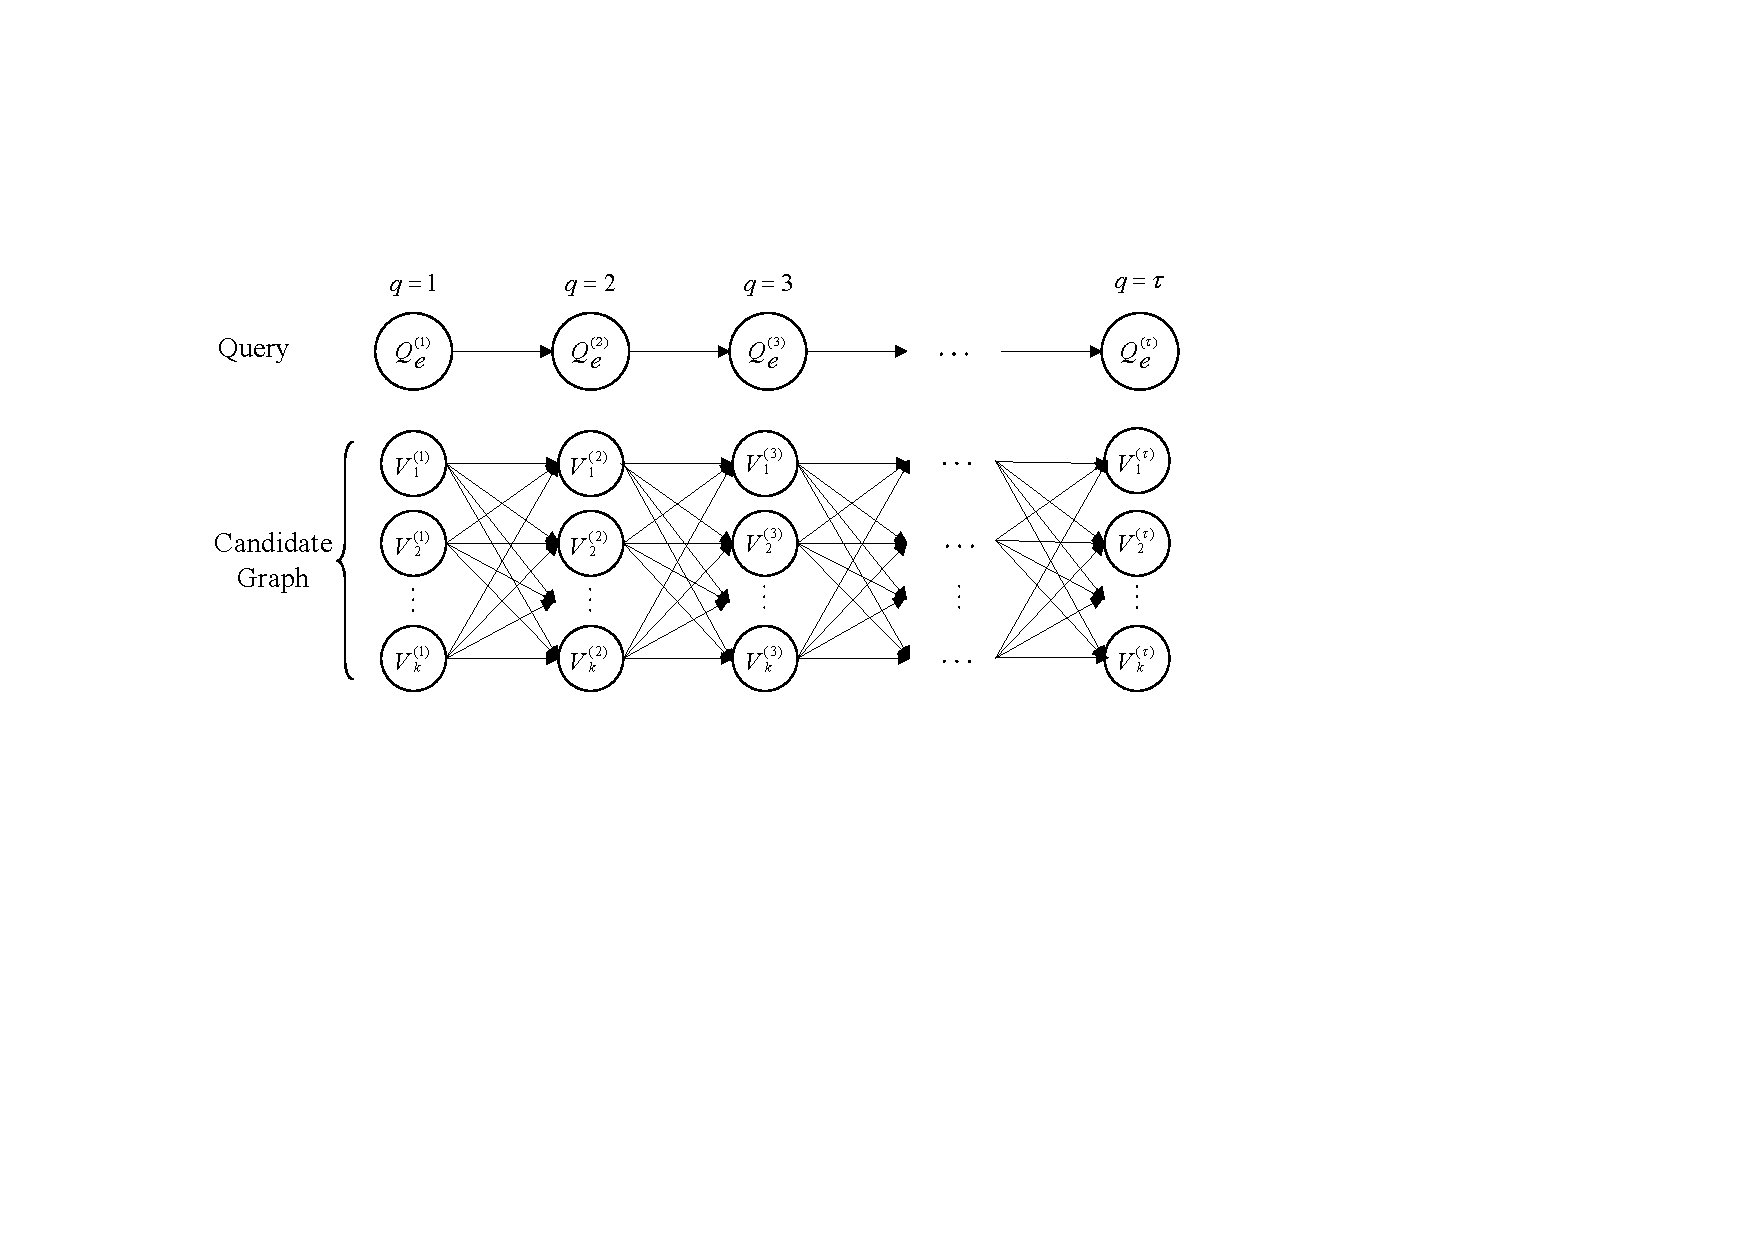
\includegraphics[width=0.90\textwidth]{data/img/dijkstra.pdf}
    \caption{用于检索的有向图}
    \label{fig:dijkstra}
\end{figure}

令$\mathcal{P}_{V_i^{(1)}\to V_j^{(\tau)}}$为连接起始节点$V_i^{(1)}$和终止节点$V_j^{(\tau)}$的路径,这里$i,j\in\{1,2,\ldots,k\}$。
在所有从第一到最后帧的可能路径中,我们找到最短路。优化目标被正式定义如下:
\begin{eqnarray}\label{eq:dijkstra}
\mathcal{P}_{opt}=\mathop{\arg\min}_{i, j} \mathop{\arg\min}_{\mathcal{P}_{V_i^{(1)}\to V_j^{(\tau)}}}
        \sum_{r\in \mathcal{P}_{V_i^{(1)}\to V_j^{(\tau)}}}\mathcal{L}(r).
\end{eqnarray}

该问题用Fibonacci堆~\cite{algorithm}的Dijkstra算法很好解决。连接最优路径$\mathcal{P}_{opt}$的所有帧构成检索序列。

我们的基于优化的方法借鉴了以往用于生成时间一致动画的工作~\cite{Kovar_Gleicher,spacetime,photobios}。我们的方法结合了时间一致性和语义对应。

\subsection{表情精炼}\label{sec:emi}
前面的检索结果有两个缺点。首先,由于我们的数据库的大小是有限的,检索的帧可能不包含和输入序列完全相同的表情。其次,数据库中的帧没完全对齐,所以检索序列包含了一些少量的时间抖动。要删除这些错误,我们的系统采用了额外的表情细化组成部分。

表情精炼的主要思路是给定$Q_n$ 和$Q_e$,中性帧和人偶师的表情帧,还有$T_n$,目标人的中性帧,我们可以直接从两个源图片中提取表情,并映射到$T_n$来合成新的面部$T_{Q_e}$。该合成的脸部,我们称之为expression mapping image(EMI),有所需的表情,但是也许没有逼真的纹理,尤其当$Q_n$ 和 $Q_e$表情差异很大的时候。另一方面,检索帧有真实的外表,但表情和$Q_e$并不完美匹配。结合EMI和检索帧,我们可以生成最终图片,有逼真的外表和精确匹配的表情。

具体说,我们首先通过把$Q_n$ 和$Q_e$的光流转移到目标帧来扭曲$T_n$。给定点$\vec{a}\in Q_n$,$\vec{a}'\in Q_e$和$\vec{b}\in T_n$ ($\vec{b}=g(\vec{a})$ 如公式~\ref{eq:map2}),我们计算点$\vec{b}'\in T_{Q_e}$ 的颜色如下:
\begin{equation}\label{eq:ratio}
c_{\vec{b}'}=c_{\vec{b}}\frac{c_{\vec{a}'}}{c_{\vec{a}}},
\end{equation}

这里$c_{\{\vec{a},\vec{a}',\vec{b},\vec{b}'\}}$分别是点$\vec{a}$, $\vec{a}'$, $\vec{b}$ and $\vec{b}'$的颜色值(我们系统中使用YCrCb颜色空间)。这里我们用比值${c_{\vec{a}'}}/{c_{\vec{a}}}$来表示颜色$c_{\vec{b}}$如ERI方法~\cite{eri}所做。在实际实施中,为了避免$\vec{b}'$有非整数坐标,我们用反向计算表情映射我们从一个整数像素$\vec{b}'\in T_{Q_e}$开始,根据$\vec{a}'=g^{-1}(b')$找到它的对应点$\vec{a}'\in Q_e$ 。通过计算\mbox{\boldmath $F$}$_{Q_e \to Q_n}$获得的光流$\Delta \vec{a}'$ 给出点$\vec{a}$的坐标。通过注册函数,我们获得点$\vec{b}=g(\vec{a})\in Q_n$的位置。然后点$\vec{b}'$ 的颜色可以依据公式\ref{eq:ratio} 计算。

\begin{figure}[htbp]
\centering
    \subcaptionbox{}{
    \label{fig:refine_driven}
    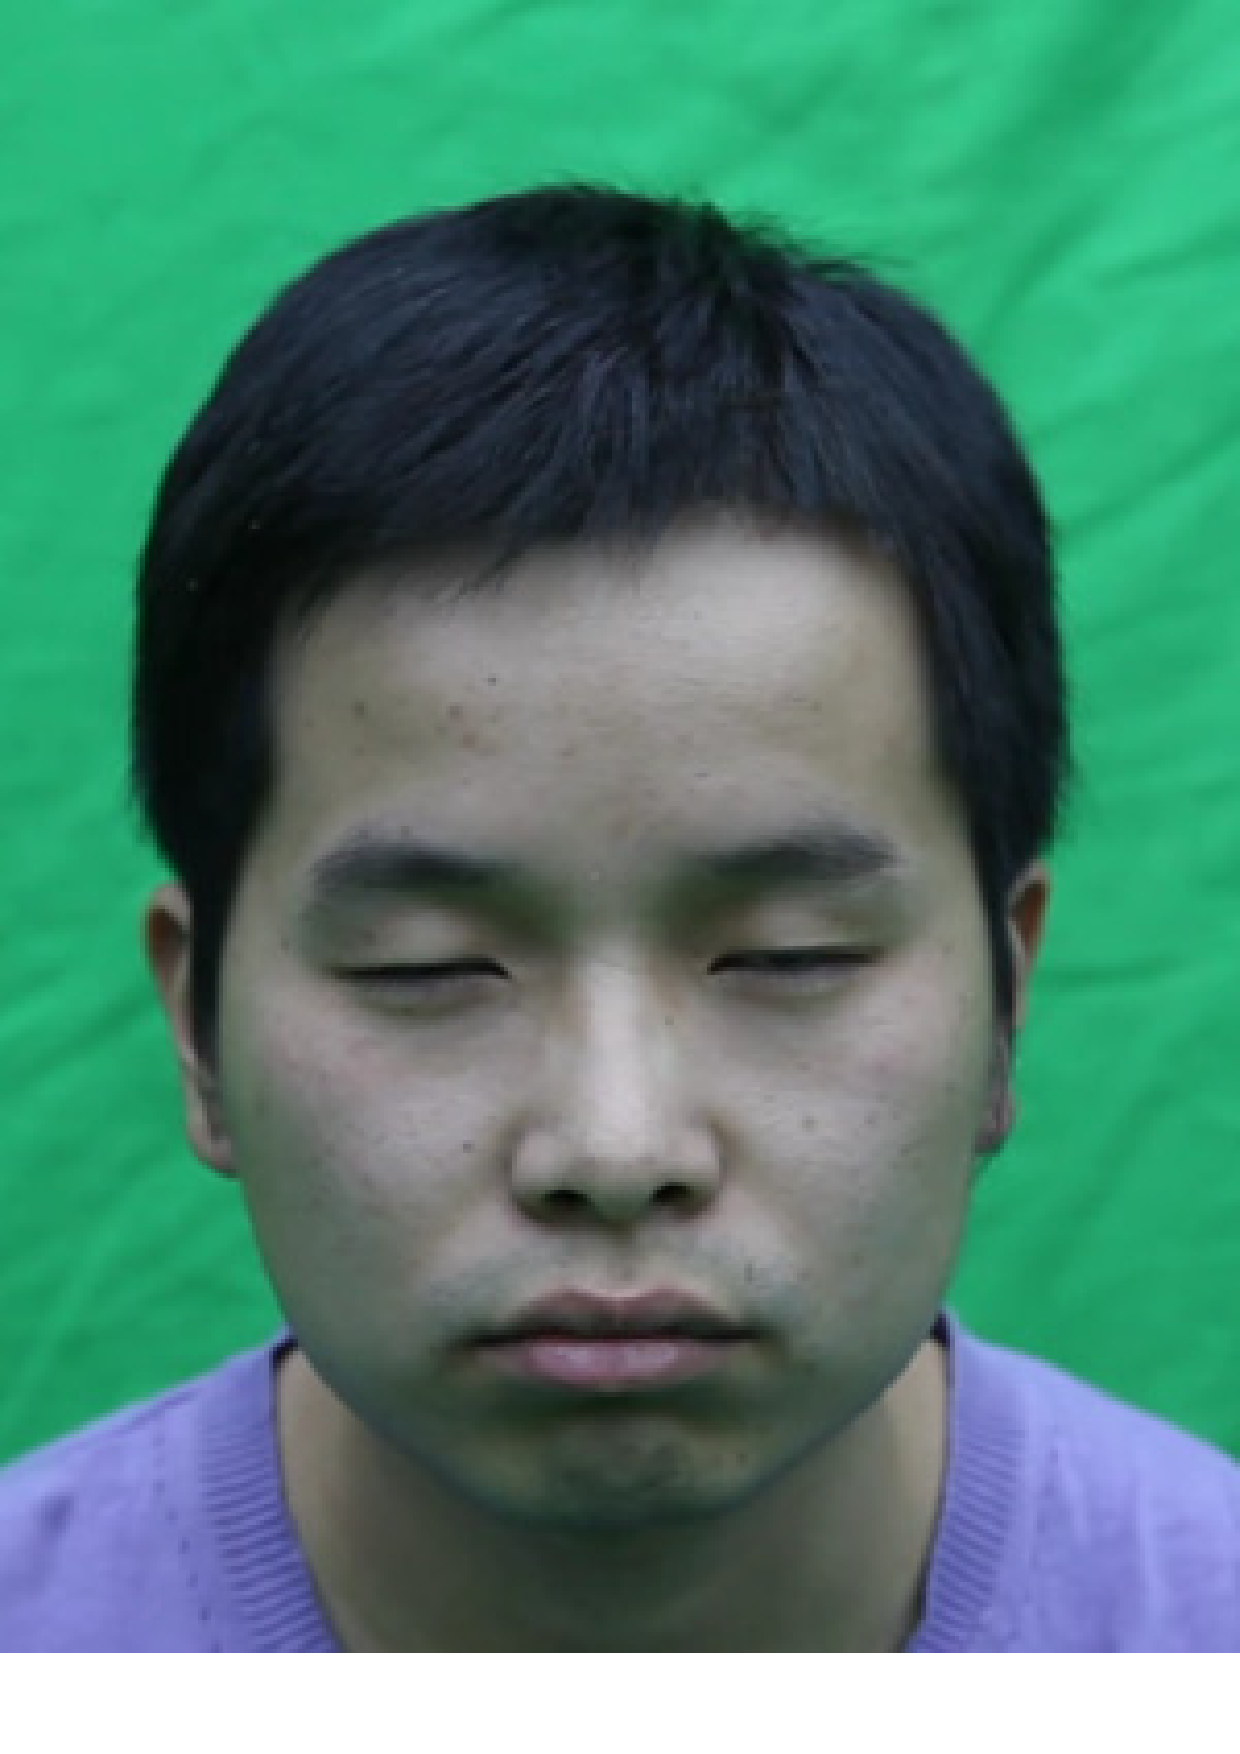
\includegraphics[width=0.23\textwidth]{data/img/refine_likai_0380_00151.pdf}}
    \subcaptionbox{}{
    \label{fig:refine_retrieval}
    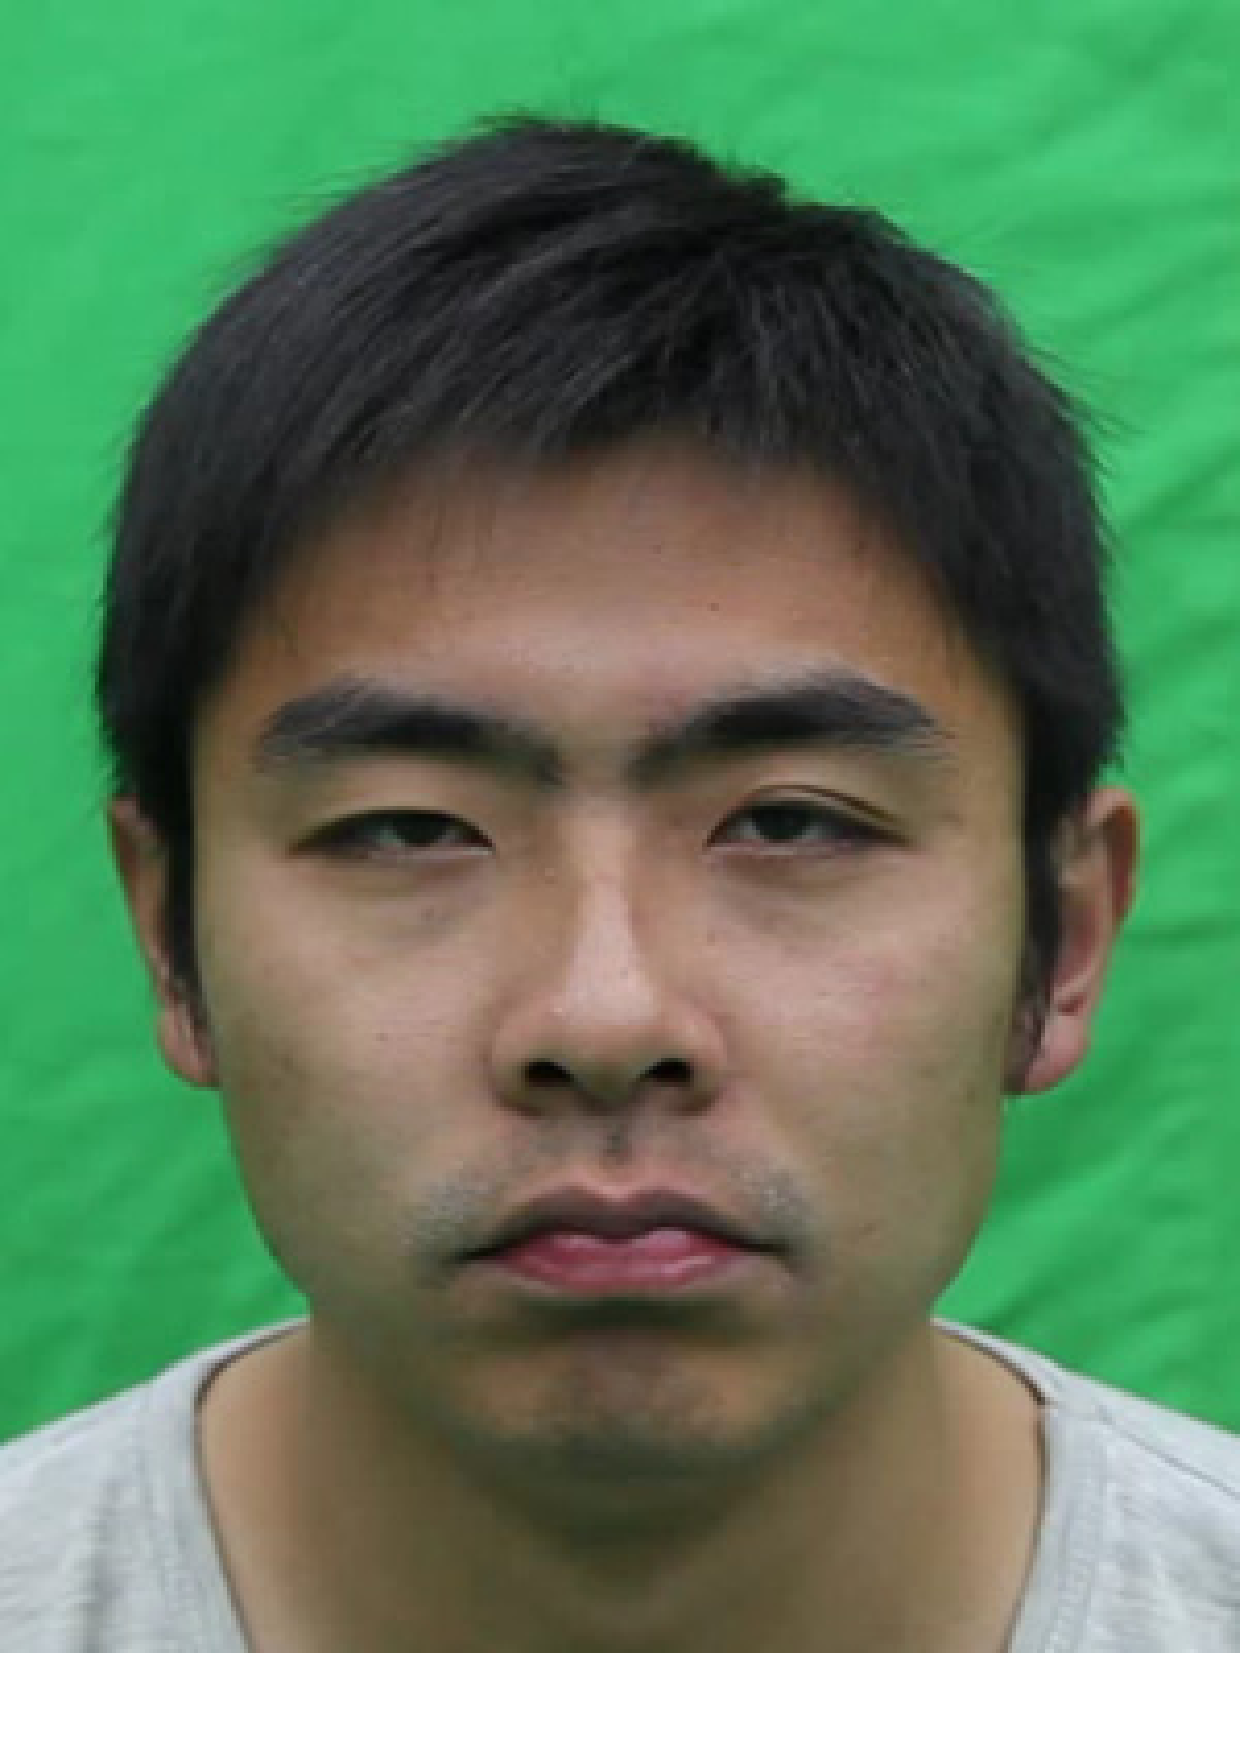
\includegraphics[width=0.23\textwidth]{data/img/refine_retrieval_00150.pdf}}
    \subcaptionbox{}{
    \label{fig:refine_emi}
    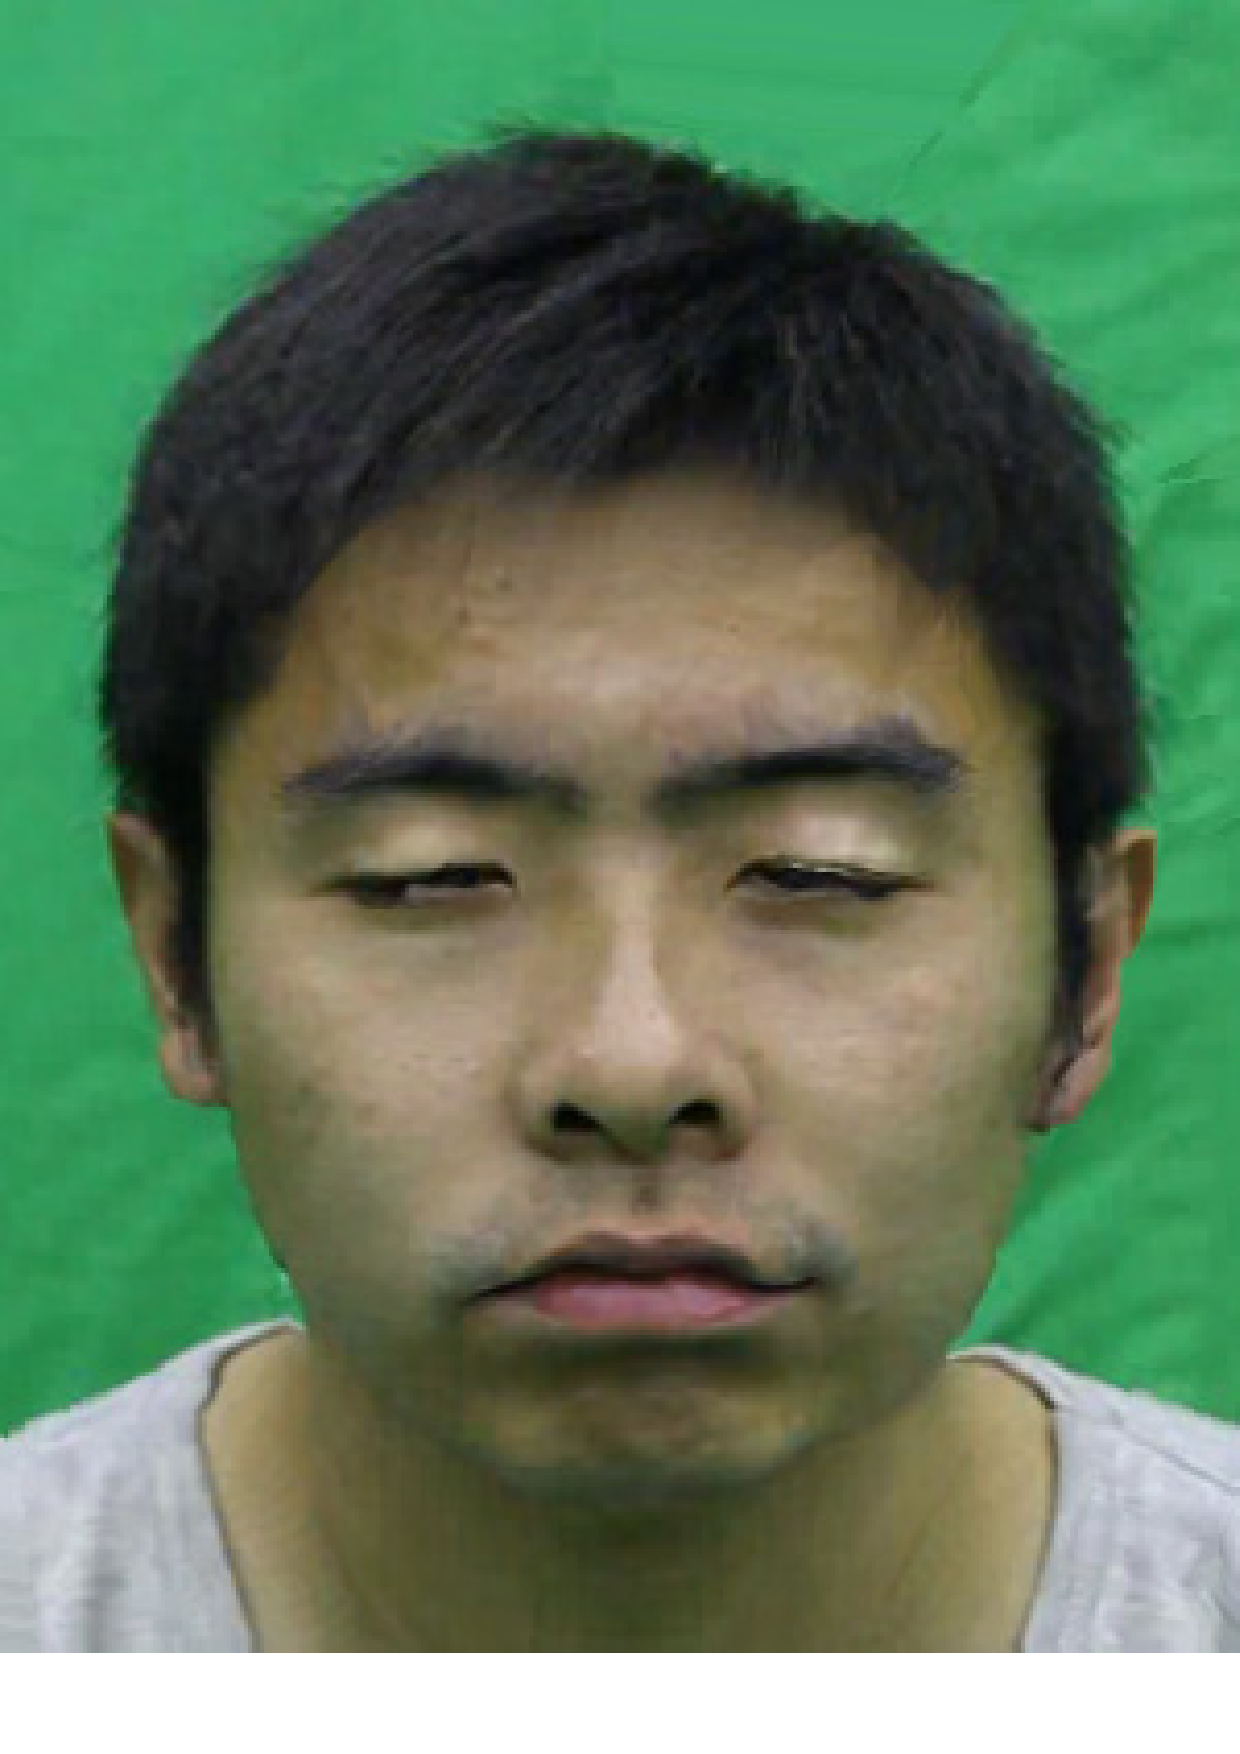
\includegraphics[width=0.23\textwidth]{data/img/refine_EMI_00151.pdf}}
    \subcaptionbox{}{
    \label{fig:refine_final}
    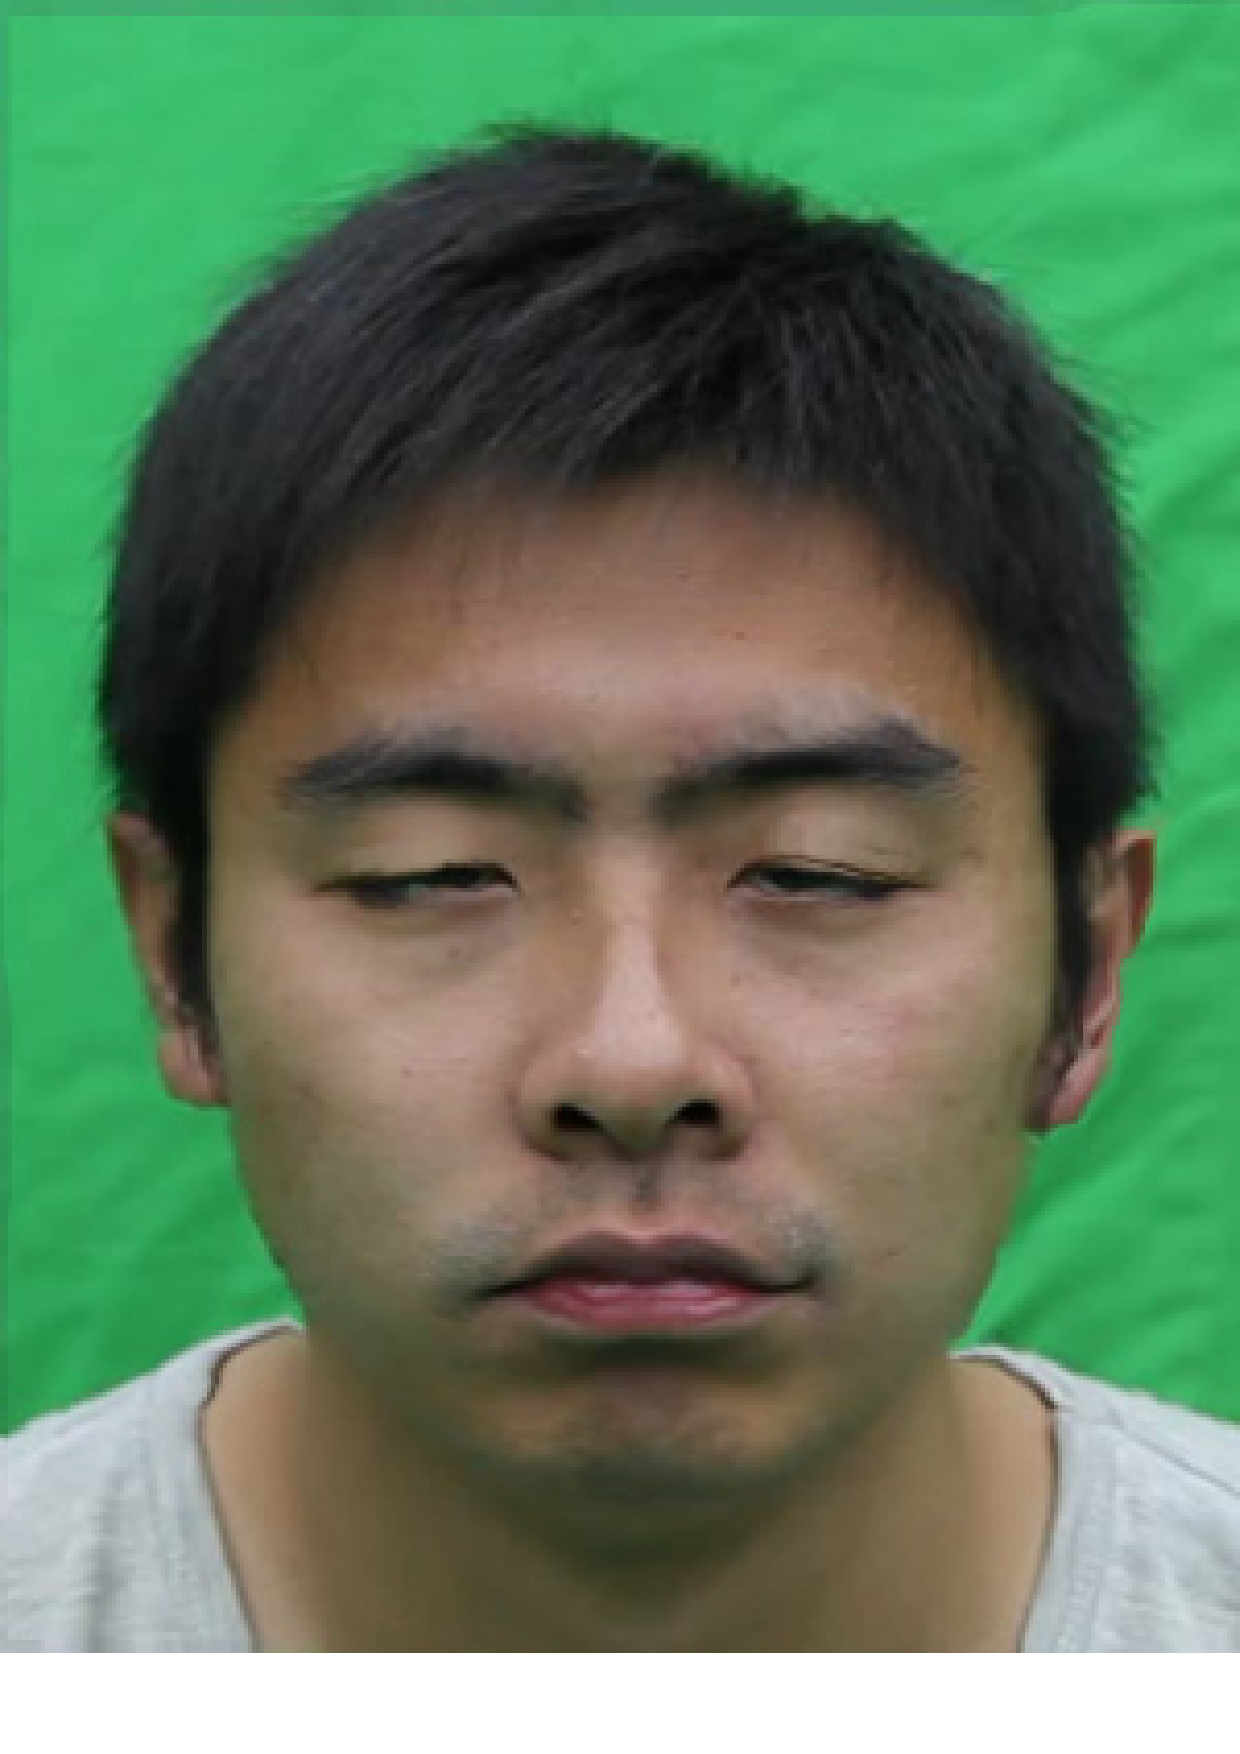
\includegraphics[width=0.23\textwidth]{data/img/refine_combine_00150.pdf}}
    \caption{表情精炼。 (a) 查询帧。 (b) 检索帧。 (c) 表情映射图片。 (d) 最终结果。}
    \label{fig:refine}
\end{figure}

最终,我们计算每一帧时的EMI和检索结果的光流,并利用光流扭曲检索图像至EMI。如图~\ref{fig:refine}所示,最终合成结果不只有从检索帧继承来的真实的外表,还有由EMI图像继承来的和查询帧匹配的正确表情。
\section{结论和讨论}
\begin{figure}[htbp]
\centering
    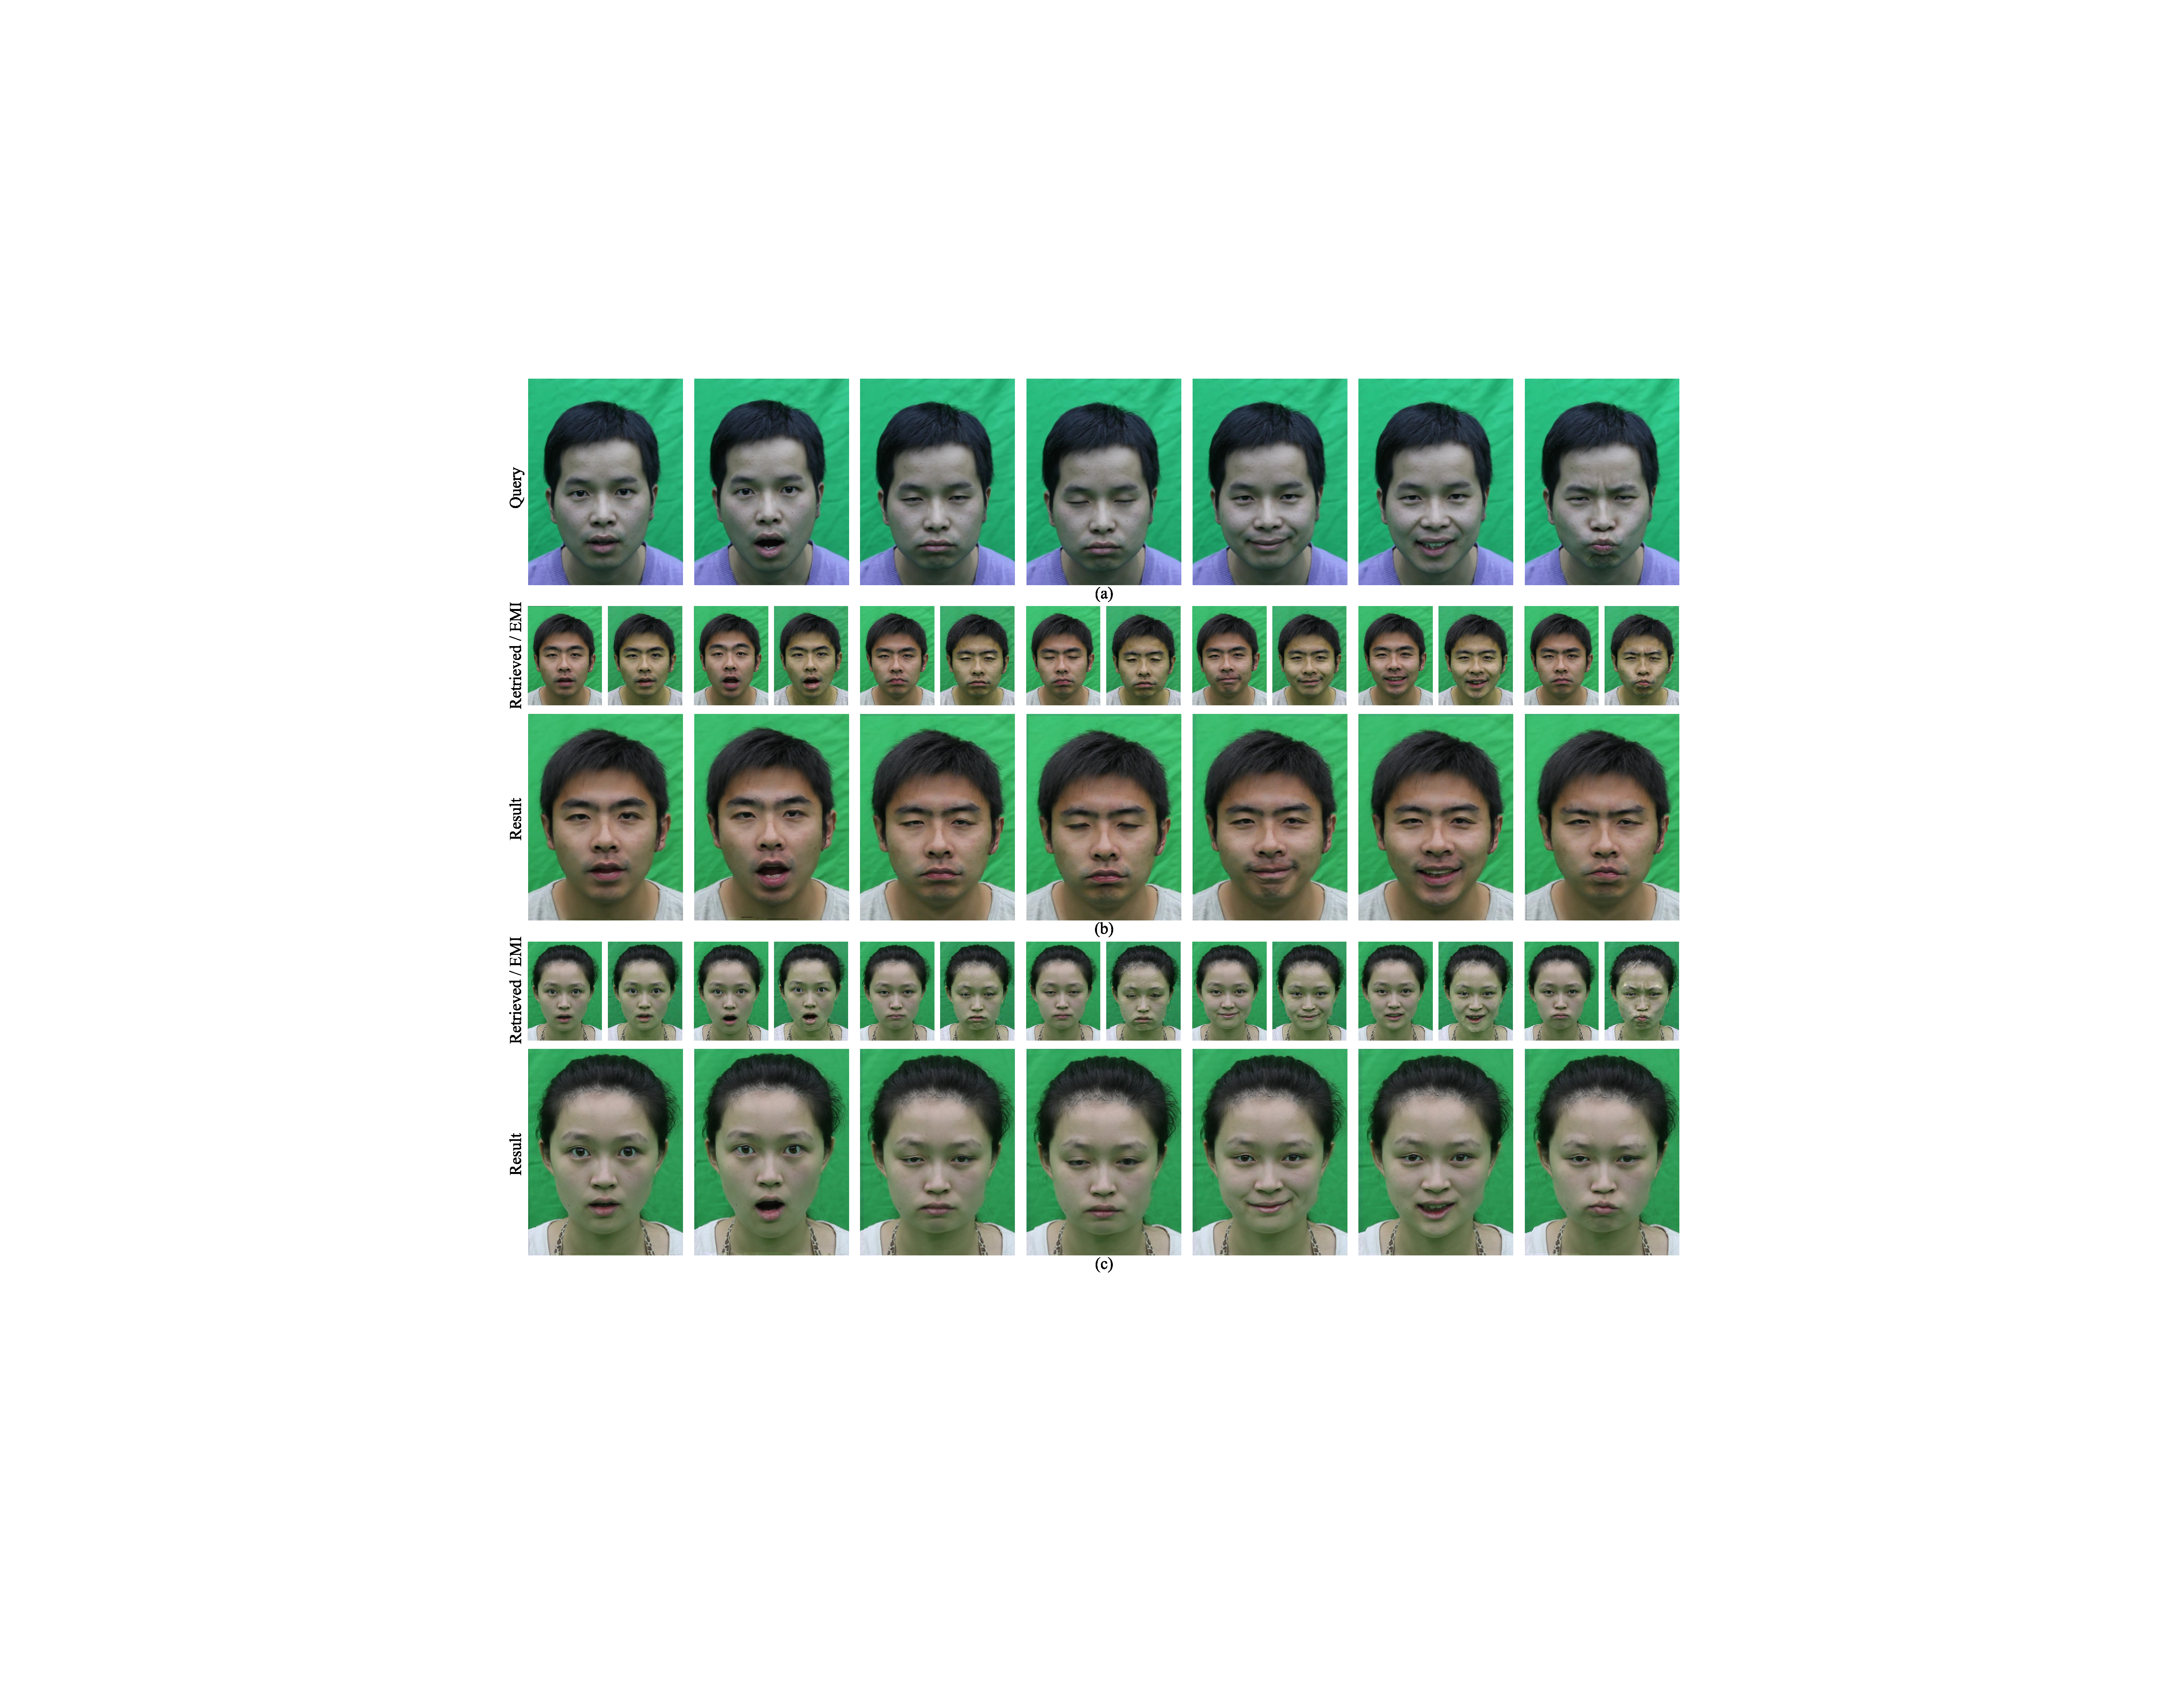
\includegraphics[width=0.9\textwidth]{data/img/likai2xf_jyy.pdf}
    \caption{在目标 $T1$ 和 $T2$ 上运行的查询序列的结果。 (a) 普通查询帧
    (b) (第一行)检索和EMI帧(分别是左和右);(第二行)目标 $T1$ 的最终合成帧。 (c) 目标 $T2$ 的检索、EMI帧和Retrieved最终合成帧。}
    \label{fig:result12}
\end{figure}

\subsection{实验}
我们评估了三个数据库系统。其中两个是我们采集的,这两个主题一个是男性,一个女性,他们被要求表现6个基本表情:愤怒,厌恶,惊讶,恐惧,快乐和悲伤。每个数据库都是25fps拍摄,包含约1500帧。第三个数据库是从Extended Cohn-Kanade Dataset (CK+) \cite{CK+}得到的 S130 。 S130 中的11个短序列(共220帧)构成了该表情数据库。在所有试验中,我们算法的参数固定如下:$\alpha_e=\frac{0.6}{n_{e}}$, $\alpha_m=\frac{0.4}{n_m}$, $\beta_m=0.9$, $\beta_o=0.1$,
$\gamma_e=0.9$, $\gamma_v=0.1$, $k=20$, $\lambda=0.1$, $\mu=1$, $\sigma=2$,其中 $n_e$ 和 $n_m$ 分别是目标中性面眼镜和嘴巴区域的像素数量。

\subsection{结果和评估}
图~\ref{fig:result12}显示了目标 $T1$(男性)和 $T2$ (女性)由输入序列驱动的合成结果。注意我们的系统不仅在诸如笑脸和惊奇等表情在数据库中时可以合成逼真的表情,而且在诸如撅嘴且双眼紧闭的表情在数据库中没有的时候也能合成新表情。同时,最终合成的视频也是时间相干的。图~\ref{fig:result3}展示了由另一序列驱动,从来自 CK+ 数据库的S130 中合成的结果。结果表明即使只是一个小数据库我们的系统仍然效果很好。可以在补充材料中找到包括额外的快速说话重定位结果的完整的视频序列。
为了评价我们的合成结果,我们进行了包含 $34$ 个参与者的用户研究。每位参与者都被展示了四个视频,分别由 LBP 特征查询方法~\cite{eccv10},在第~\ref{sec:emi}章介绍的 EMI 方法,我们的检索策略和我们的整套算法一帧一帧查询获得。每个视频并排展示了查询和结果。在实验中,参与者被要求根据表情的真实性和一致性评价在每个结果中表情的好坏,分数从 5(非常好)到 0(一点也不好)。表~\ref{tab:userstudy} 显示了3个目标的平均分。参与者发现我们的最终结果是最好的且我们的检索策略优于在~\cite{eccv10}提出的方法。
\renewcommand{\tablename}{表}
\begin{table}[htp]
\centering
    \begin{tabular}{|l|p{1cm}|p{1cm}|p{1cm}|}
    \hline
    & $T1$ & $T2$ & S130\\
    \hline\hline
    基于 LBP 的检索 \cite{eccv10} & 1.20 & $1.50$ & $1.38$\\
    我们的检索 & $2.49$ & $3.00$ & $2.56$\\
    EMI & $2.89$ & $1.91$ & $3.35$\\
    我们的整套系统 & $\mathbf{4.02}$ & $\mathbf{4.56}$ & $\mathbf{4.08}$\\
    \hline\hline
    $p$ 值 & $0.002$ & $0.005$ & $0.0001$ \\
    \hline
    \end{tabular}
    \caption{用户研究结果。该结果在统计上是有意义的,使用了单变量方差分析,$p$-value $<0.01$。}
    \label{tab:userstudy}
\end{table}

\subsection{局限性}
我们目前的系统只针对正面脸部表情合成设计。可能会扩展系统在大旋转角下运行,通过稀疏相机阵列采集数据。如此我们需要估计表情和输入帧的3D脸部。此外,需要视图变形技术~\cite{ViewMorphing}来在不同视角查看脸部,以在所需姿态生成面部表情。

另一个限制是,当表情很极端,传统的光溜方法无法精确捕捉表情差异。除了调查更好的脸部光流技术,另一个解决方案是为每个特征使用多个预先对其的脸部图像而不只是在我们现有系统中使用单一中性面。

\begin{figure*}[htbp]
\centering
    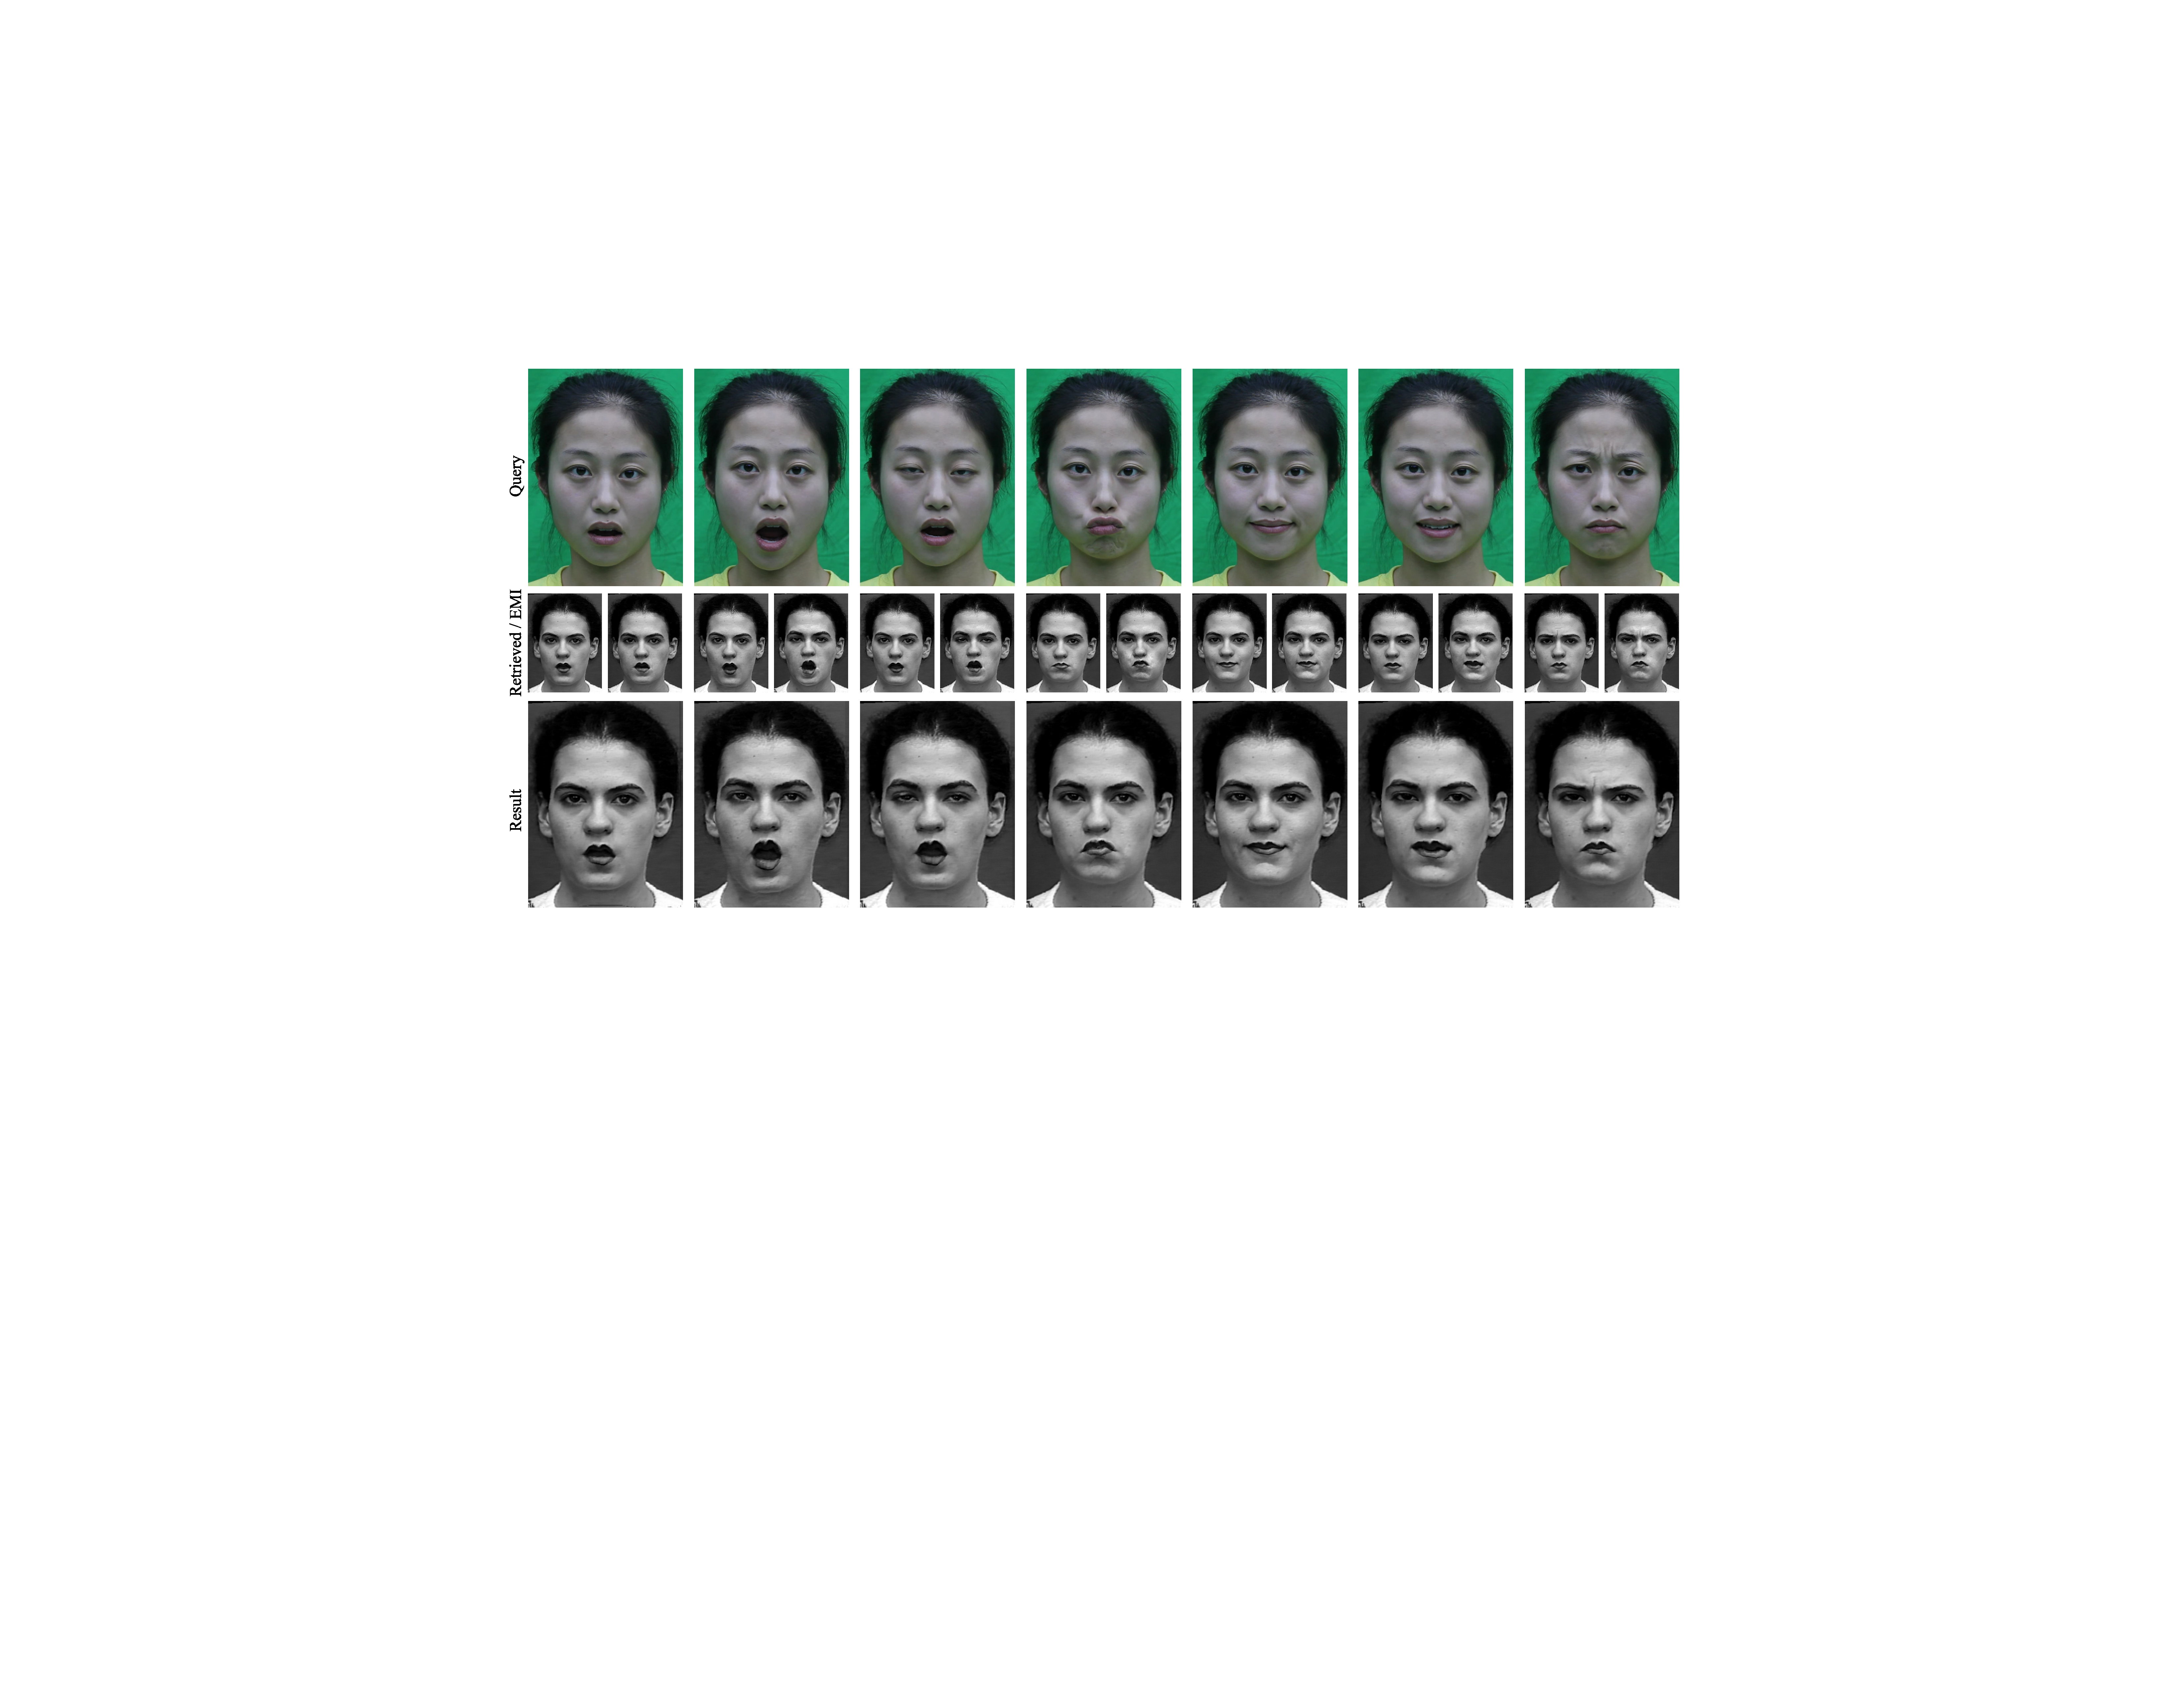
\includegraphics[width=0.90\textwidth]{data/img/liwen2S130.pdf}
    \caption{在来自CK+的S130中由查询序列2获得的结果。 (顶部)查询帧。(中部)检索帧和EMI 帧(分别是左和右)。(底部)最终合成帧。}
    \label{fig:result3}
\end{figure*}

\section{结论}

我们提出了一种数据驱动的方法来用一个人的面部表情视频对目标人脸合成真实的面部动画。我们的系统采用了新颖的时空表情距离度量,可以准确地测量视频中不同的人相似的表情。我们也提出了最短路径优化的检索策略来平衡在最终视频的表情相似性和时间连续性。和那些直接表情映射相比,通过变换检索到的视频帧进一步改善了表情相似性。用户研究结果表明,我们的系统可以产生很高的保真度和时间上一致的面部动画。

\section*{致谢}
作者要感谢和王瑞平,邓岳,索津莉的讨论,评审和领导建设性的意见。这项研究由国家自然科学基金项目支持(第61035002号,第61073072号,第60933006号)。

\setcounter{NAT@ctr}{0}%
\renewcommand{\refname} {参考文献}
{\small
\bibliographystyle{ieee}
\pagestyle{empty}
\bibliography{egbib}
}
